\chapter{极小曲面的基本性质}
极小曲面起源于下面的问题:
\begin{question*}
    给定简单闭曲线$\gamma \subset \R^3$, 是否存在以$\gamma$为边界的面积最小的曲面? 即, 寻找曲面$\Sigma, \partial \Sigma = \gamma$, 使得对于任意满足$\partial \Sigma' = \gamma$的曲面$\Sigma'$, 都有
    \begin{equation*}
        \Area(\Sigma) \le \Area(\Sigma')
    \end{equation*}
\end{question*}
这个问题现在被称为Plateau问题(最早由Langrage提出). 1920-30s年代, 这个问题被 Rado 和 Douglas 解决(Douglas 也因为在 Plateau 问题上的工作而获得第一届Fields奖).
\section{极小曲面方程}
每个曲面都可以局部地表示为函数的图像的形式, 因此我们首先来研究可以作为函数图像的曲面. 设$\Sigma$是面积最小的曲面, 且
\begin{equation*}
    \Sigma= \G(u)= \{(x,u(x))\mid x \in \Omega\}
\end{equation*}
其中, $\Omega$ 是给定的有界区域, $u \in \CC(\Omega)$. 若使得$\G(u)$面积最小, 那么对于任意$\phi \in \CC(\Omega)$ 及$t \in \R$,
\begin{equation}
    \Area(\G(u)) \le \Area(\G(u+t\phi))
\end{equation}
于是, 我们有
\begin{equation}
    \ddt(\Area(\G(u+t\phi)))\mid_ {t=0}=0
\end{equation}
直接计算可知
\begin{equation}
    \begin{split}
        \Area(\G(u+t\phi)) &= \int_\Omega \sqrt{1+\abs{Du+tD\phi}^2} \\
                          &= \int_\Omega \sqrt{1+\abs{Du}^2}+t\frac{\inner{Du}{D\phi}}{\sqrt{1+\abs{Du}^2}} + o(t)
    \end{split}
\end{equation}
因此, $\forall \phi \in \CC(\Omega)$, 成立
\begin{equation}
    \begin{split}
        \ddt \Area(\G(u+t\phi))\mid _{t=0} & = \int_\Omega \frac{\inner{Du}{D\phi}}{\sqrt{1+\abs{Du}^2}} \\
        &=- \int_\Omega \phi \div \frac{Du}{\sqrt{1+\abs{Du}^2}} =0
    \end{split}
\end{equation}
下面的方程便称为极小曲面方程(MSE).
\begin{equation}
    \div \frac{Du}{\sqrt{1+\abs{Du}^2}} =0
\end{equation}
\begin{remark}
    一个曲面是否局部地满足MSE, 跟我们选取的坐标表示是没有关系的.
\end{remark}
显然地, 一个函数$u$满足极小曲面方程只是$\G(u)$面积最小的必要条件, 是否有可能是充分条件? 我们有下面的两个结论.
\begin{proposition}\label{mse_min1}
    设$\Omega \subset \R^n$是有界区域, $u \in C^2(\Omega)\cap C(\overline{\Omega})$. 设$u$满足MSE. 设$\Sigma \subset \Omega \times \R$且$\partial \Sigma = \partial \G(u)$. 则有
    \begin{equation}
        \Area(\G(u)) \le \Area(\Sigma)
    \end{equation}
\end{proposition}
\begin{proof}
    记$\vec{n}= \frac{\partial_{n+1}-Du}{\sqrt{1+\abs{Du}^2}}$为$\G(u)$的单位法向(这里我们将$\vec{n}$自然地扩张到$\R^{n+1}$上). 由于$u$满足MSE, 则$\div(\vec{n})=0$. 设$dx$是$\R^{n+1}$中的体积形式, 定义$n-$ 形式 $\omega=i_*^{\vec{n}}dx$如下, 对于任意向量场 $X_1,X_2, \cdots,X_n$:
    \begin{equation}
        \omega(X_1,X_2,\cdots,X_n)=dx(X_1,X_2,\cdots,X_n,\vec{n})
    \end{equation}
    显然地, $\omega$是多重线性的反对称张量, 即是一个$n-$形式.  现在验证$\omega$有如下性质:
    \begin{enumerate}
        \item $d\omega=0$.
        \item $\forall$ 单位向量场 $e_1,e_2,\cdots,e_n$, 成立$\omega(e_1,e_2,\cdots,e_n) \le 1$. 并且等号成立当且仅当$e_1,e_2,\cdots,e_n$形成$T\Sigma$的标准正交基.
    \end{enumerate}
    性质(1)由基本公式$d(i_*^{\vec{n}}dx)=\div(\vec{n})dx$ 可知.  为了验证性质 (2), 设$V=span(e_2,e_3,\cdots,e_n,\vec{n})$. 将$e_1$分解为平行于$V$和垂直于$V$的部分, $e_1=e_1^T+e_1^{\perp}$. 则
    \begin{equation}
        \omega(e_1,\cdots,e_n,\vec{n})=\det([e_1^{\perp}, e_2,\cdots,e_n,\vec{n}])
    \end{equation}
    同样的相对于空间$span(e_3,\cdots,e_n,\vec{n})$, 分解$e_2$. 这样一直做下去, 最终有
    \begin{equation}
        \omega(e_1,\cdots,e_n,\vec{n})=\det([e_1^\perp, e_2^\perp,\cdots,e_n^\perp,\vec{n}]) \le 1
    \end{equation}
    等号成立当且仅当每一步地分解中, $e_i^T=0$. 因此性质(2)成立. 性质(2)的两个直接推论是, 当$\omega$限制在$\G(u)$上时, $\omega$恰好为$\G(u)$上的面积形式. 当$\omega$限制在$\Sigma$上时, $\omega \le d\Sigma$(这里指的是$\omega=f(x)d\Sigma, \abs{f}\le 1$). 
    \par 由于 $H_n(\Omega \times \R)=H_n(\Omega)=\{0\}$, 则存区域$W \subset \Omega \times \R$使得$\partial W=\G(u)-\Sigma$. 由Stokes公式可知
    \begin{equation}
        0=\int_W d\omega= \int_{\G(u)}w-\int_{\Sigma}w \ge \Area(\G(u)) - \Area(\Sigma)
    \end{equation}
\end{proof}
\begin{proposition}\label{mse_min2}
    设$\Omega \subset \R^n$是有界凸区域. 设$u \in C^2(\Omega) \cap C(\overline{\Omega})$. 设$u$满足MSE. 设$\Sigma\subset \R^{n+1}$且$\partial \Sigma = \partial \G(u)$, 则有
    \begin{equation}
        \Area(\G(u)) \le \Area(\Sigma)
    \end{equation}
\end{proposition}
\begin{proof}
    设$P:\R^{n+1} \subset \overline{\Omega} \times \R$是 nearest point projection, 即$\forall x \in \R^{n+1}$, $P(x)$是$\overline{\Omega}\times \R$中离 $x$最近的点. 由于$\Omega$是凸的, $P(x)$存在且唯一. 易知$\abs{P(x)-P(y)} \le \abs{x-y}$, 即$P$是$1-Lipschitz$连续的, 在它的作用下, 长度,面积,体积等都会减少(不增). 由于$P(\Sigma) \subset \overline{\Omega} \times \R$, 我们可以应用命题\eqref{mse_min1}
    \begin{equation}
        \Area(\Sigma) \ge \Area(P(\Sigma)) \ge \Area(\G(u))
    \end{equation}
\end{proof}
命题\eqref{mse_min1}中的证明还可以得到下面的结论:
\begin{corollary}
    设$u: \Omega \to \R$满足MSE. 设$B_r \subset \Omega \times \R$. 则有
    \begin{equation}
        \Area(B_r \cap \G(u)) \le \frac{1}{2} \Area(\partial B_r)
    \end{equation}
\end{corollary}
\begin{proof}
    设$B_r$在$\Omega$中的投影为$B'$. 显然$B'$是凸集. $\partial B_r \cap \G(u)$将$\partial B_r$分成两部分, 分别记为$S^+, S^-$. 设$\Sigma'= B'\times \R \cap \Sigma$. 由命题\eqref{mse_min2}可知, 
    \begin{align}
        &\Area((\Sigma'-B_r \cap \Sigma) \cup S^+) \ge \Area(\Sigma') \\
        &\Area((\Sigma'-B_r \cap \Sigma) \cup S^-) \ge \Area(\Sigma')
    \end{align}
    而这等价于
    \begin{align}
        &\Area(S^+) \ge \Area(B_r \cap \Sigma)  \\
        &\Area(S^-) \ge \Area(B_r \cap \Sigma) 
    \end{align}
\end{proof}
\section{第一变分公式} \label{sec_first_variation}
设$(\M^n,g)$是黎曼流形, $\Sigma^{n-1}\subset \M$是$n-1$维子流形. 我们采取的记号如下
\begin{itemize}
    \item $X^T,X^\perp$: 切向量$X \in T_pM$在$T_p\Sigma$上的切向及法向分量.
    \item $T_p^\perp \Sigma$:=$\{X\mid X\in T_pM, X\perp T_p\Sigma\}$. $\Sigma$在$p$点处的法丛.
    \item $\nabla,\nabla_\Sigma$: $\M$及$\Sigma$上的Levi-Civita联络. $\nabla_\Sigma=\nabla^{T}$.
    \item $A/\II$: $\Sigma$在$\M$中的向量值与标量值第二基本形式. $A(X,Y)=(\nabla_XY)^\perp$. $\II(X,Y)=\inner{A(X,Y)}{\vec{n}}$. $\vec{n}$为给定的单位法向.
    \item $\vec{H}$: $\Sigma$的平均曲率向量. $\vec{H}(p)=\Tr(A)=\sum_{i}^{n-1}A(e_i,e_i)$, $\{e_i\}$是$T_p\Sigma$的标准正交基.
    \item ${H}$: $\Sigma$的平均曲率. $H=\inner{\vec{H}}{\vec{n}}$, $\vec{n}$为$\Sigma$的单位法向.
    \item $\div_\Sigma X$: $X \in TM$在$\Sigma$上的散度. $\div_\Sigma X=\sum_{i=1}^{n-1}\inner{\nabla_{e_i}X}{e_i}$. $\{e_i\}$是 $T\Sigma$的标准正交基(验证这个定义与基的选取无关). 需要注意 , 这里$X$可以定义在$TM$上, 而不仅仅是$T\Sigma$上. 散度算子满足如下的Lebniez公式:
    \begin{equation}
        \div_\Sigma(fX)=f\div_\Sigma(X)+\inner{\nabla_\Sigma f}{X}
    \end{equation}
\end{itemize}
设$F(x,t): \Sigma \times (-\epsilon, \epsilon) \to \M$是曲面$\Sigma$的一个变分(连续形变)满足
\begin{enumerate}
    \item $F(x,0)=x$.
    \item $\forall x \in \partial \Sigma, F(x,t)=x$.
\end{enumerate}

\begin{figure}[ht]
	\centering
	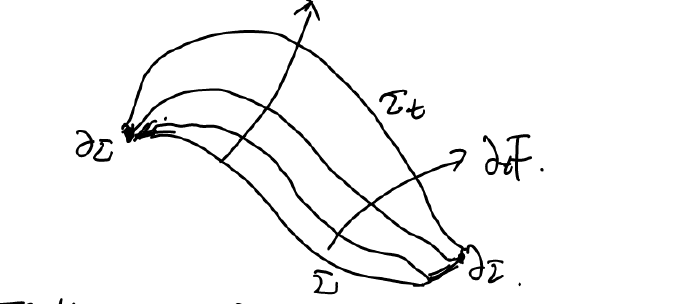
\includegraphics[scale=0.8]{images/variation.png}
	\caption{曲面的变分}
	\label{variation_p}
\end{figure}


\begin{remark}
    我们假设$\epsilon$足够小时, $F$是$\Sigma \times (-\epsilon,\epsilon)$到它的像之间的同胚. 选定$\Sigma$上的一组局部坐标系$(x^i)$. 以后我们将$\partial_t$与 $dF\partial_t$等同, 将$\partial_i$与$dF\partial_i$等同, 并分别记作$\partial_t F$与$\partial_i F$.
\end{remark}
设$\Sigma$上的度量为$g$, $\Sigma_t$上的度量记为 $g(t)$. 则$g_{ij}(t)=\inner{\partial_iF}{\partial_jF}$. 在这些记号下, 
\begin{equation}
    \Area(\Sigma_t)=\int_\Sigma \sqrt{\det g(t)}dx
\end{equation}
\begin{equation}
    \ddt \Area(\Sigma_t)=\int_\Sigma \ddt \sqrt{\det g(t)}dx
\end{equation}
\par 现在我们来求面积的第一变分. 首先证明一个引理.
\begin{lemma}
    设$A=[a_{ij}]$是 $n \times n$矩阵. 将$\det A$看作$n^2$个变量$(a_{ij})$的函数. 则$d\det A= A^{ij}da_{ij}$. $A^{ij}$是$A$的代数余子式.
\end{lemma}
\begin{proof}
    由行列式的拉普拉斯展开, 我们知道 $\forall i, \det A= \Sigma_{j}A^{ij}a_{ij}$. 注意到$A^{ij}$与${a_{ij}}$无关, 则有$\frac{\partial \det A}{\partial a_{ij}}=A^{ij}$.
\end{proof}
\begin{corollary} \label{det_jacobi}
    设$A_t=[a_{ij}(t)]$. 则$\ddt \det A_t=\det A_t \Tr(A_t^{-1}\ddt A_t)$.
\end{corollary}
固定一个点$p \in \Sigma$并选取$p$点处的测地坐标. 以后所有计算都将在点$p$处进行.
\begin{equation}
    2\ddt \sqrt{\det g(t)}\mid_{t=0}=\Tr(g'(0))
\end{equation}
现在, 我们只需要计算$g'_{ij}(0)$即可. 根据定义, $g_{ij}(t)=\inner{\partial_iF}{\partial_jF}$. 对$t$求偏导, 则有
\begin{equation}
    \begin{split}
        \ddt g_{ij}(t)& =\nabla_{\partial_t F}\inner{\partial_iF}{\partial_jF} \\
                    & =\inner{\nabla_{\partial_t F}{\partial_iF}}{\partial_jF}+ \inner{\partial_iF}{\nabla_{\partial_tF}\partial_jF}
    \end{split}
\end{equation}
由于$\nabla_{\partial_tF}\partial_iF - \nabla_{\partial_iF} \partial_tF=[\partial_tF,\partial_iF]=dF[\partial_t,\partial_i]=0$, 则有

\begin{equation}
    \begin{split}
        \ddt g_{ij}(t) & =\inner{\nabla_{\partial_i F}{\partial_tF}}{\partial_jF}+ \inner{\partial_iF}{\nabla_{\partial_jF}\partial_tF}
    \end{split}
\end{equation}
因此,
\begin{equation}
    \Tr(g'(0))=\sum_i 2\inner{\nabla_{\partial_iF}\partial_tF}{\partial_iF} \mid_{t=0}=2\div_\Sigma \partial_tF\mid_{t=0}
\end{equation}
若记$\omega_t$为$\Sigma_t$上的体积形式, 那么上面的等式可以写为
\begin{equation} \label{first_variation_local}
    \ddt \omega_t =(\div_\Sigma \partial_t F)\omega_t
\end{equation}
积分后便有
\begin{equation}
    \ddt \Area(\Sigma_t)\mid_{t=0}=\int_\Sigma \div_\Sigma \partial_t F
\end{equation}
而$\forall X \in TM$, 由于
\begin{equation}
    \nabla_{\partial_i}\inner{X^\perp}{\partial_j}=0=\inner{\nabla_{\partial_i}X^\perp}{\partial_j}+\inner{X^\perp}{\nabla_{\partial_i}\partial_j}
\end{equation}
以及 
\begin{equation}
    \div_\Sigma(X^\perp)=\sum_i\inner{\nabla_{\partial_i}X^\perp}{\partial_i}=-\sum_i\inner{X^\perp}{\nabla_{\partial_i}\partial_i}=-\inner{X^\perp}{\vec{H}}
\end{equation}
另外由于$\partial_tF|_{\partial \Sigma}=0$, 由散度定理可知
\begin{equation}
        \int_\Sigma \div_{\Sigma}(\partial_tF)^T =0.
\end{equation}
综上,我们有
\begin{equation}
    \begin{split}
        \ddt \Area(\Sigma_t)\mid_{t=0} & = \int_\Sigma \div_{\Sigma}(\partial_tF)^\perp + \int_\Sigma \div_{\Sigma}(\partial_tF)^T \\
        &=-\int_\Sigma\inner{\partial_tF}{\vec{H}}
    \end{split}
\end{equation}
因此, 若要使得曲面$\Sigma$的任意变分都不减小曲面的面积, 则$\Sigma$的平均曲率必定为0. 现在我们得到以下的定义:
\begin{definition}
    称$\Sigma^{n-1} \subset \M^n$是极小曲面, 如果$H_\Sigma=0$.
\end{definition}
\section{曲面上的坐标函数}
设$\Sigma^{n-1} \subset \R^n$是光滑曲面. 设$\XX=(X^1,X^2,\cdots,X^n)$为$\R^n$上的坐标函数在$\Sigma$上的限制. $\XX$的一些性质如下.
\begin{enumerate}
    \item $\nabla_\Sigma \abs{\XX}^2=2\XX^T$,$\nabla_\Sigma \abs{\XX}=\frac{\XX^T}{\abs{\XX}}$.
    \item $\Delta_\Sigma \XX=(\Delta_\Sigma X^1, \Delta_\Sigma X^2, \cdots, \Delta_\Sigma X^n)= \vec{H}_\Sigma$.
    \item $\Delta_\Sigma \abs{\XX}^2 = 2(n-1)+2\inner{H}{\XX^\perp}$.%2H\abs{\XX^\perp}$.
\end{enumerate}
\begin{proof}
    性质(1)根据定义直接可以得到.
    \par 对于性质(2), 首先需要注意, $\Delta_\Sigma \XX=(\Delta_\Sigma X^1, \Delta_\Sigma X^2, \cdots, \Delta_\Sigma X^n)$, 是在对每个分量求Laplace.  设$(\partial_i)$是$\R^n$的标准正交基. 我们注意到: 对于任意向量$Y=Y^i\partial_i \in \R^n$,
    \begin{equation}
        \nabla_Y\XX=Y^iX^j\nabla_{\partial_i}\partial_j+Y^i\partial_i(X^j)\partial_j=Y. 
    \end{equation}
    (上面的等式实际上就是$\nabla \XX =d\XX= Id$, 也可记为$Y(\XX)=Y$,  即对函数 $\XX$在$Y$方向求偏导). 取$T\Sigma$上的标准正交基$(e_i)$. 设$X^k$是$\XX$的第$k$个分量. 则$\forall Y \in T\Sigma$, 
    \begin{equation}
        \nabla^\Sigma_Y X^k= \inner{\nabla^\Sigma X^k}{Y} = \inner{\nabla X^k}{Y} = Y(X^k). 
    \end{equation}
    于是有
    \begin{equation}
        \begin{split}
            \Delta_\Sigma X^k &= \sum_i (\nabla^\Sigma_{e_i}\nabla^\Sigma_{e_i} X^k -\nabla^\Sigma_{\nabla^\Sigma_{e_i}e_i} X^k) \\
            &= \sum_i(e_ie_i X^k - (\nabla_{e_i}e_i)^T X^k).
            %&= \Tr A = \vec{H}
        \end{split}
    \end{equation}
    因此, 我们有
    \begin{equation}
        \begin{split}
            \Delta_\Sigma \XX  &= \sum_i(e_i(e_i \XX) - (\nabla_{e_i}e_i)^T \XX) \\
            &= \sum_i(\nabla_{e_i}e_i - (\nabla_{e_i}e_i)^T )\\
            &= \Tr A = \vec{H}.
        \end{split}
    \end{equation}
%    \begin{equation}
%        \begin{split}
%            \Delta_\Sigma \XX &= \sum_i (\nabla^\Sigma_{e_i}\nabla^\Sigma_{e_i}\XX-\nabla^\Sigma_{\nabla^\Sigma_{e_i}e_i}\XX) \\
%            &= \sum_i(\nabla_{e_i}e_i - (\nabla_{e_i}e_i)^T )\\
%            &= \Tr A = \vec{H}
%        \end{split}
%    \end{equation}
    \par 对于性质(3),
    \begin{equation}
        \Delta_\Sigma\abs{\XX}^2=\div_\Sigma(\nabla_\Sigma\abs{\XX}^2) = 2\div_\Sigma(\XX^T)=2\div_\Sigma(\XX)-2\div_\Sigma(\XX^\perp)
    \end{equation}
    分别计算这两项,则有
    \begin{equation}
        \div_\Sigma(\XX^\perp)=\sum_i \inner{\nabla_{e_i}\XX^\perp}{e_i}=-\sum_i\inner{\XX^\perp}{\nabla_{e_i}e_i}=-\inner{\XX^\perp}{\vec{H}}%=-\abs{X^\perp}H
    \end{equation}
    \begin{equation}
        \div_\Sigma(\XX)=\sum_i \inner{\nabla_{e_i}\XX}{e_i}=\sum_i\inner{e_i}{e_i}=n-1
    \end{equation}
    综合以上三个等式即可知性质(3).
\end{proof}
\begin{corollary} \label{coordinate_h}
    设$\Sigma^{n-1}\subset \R^n$. 则$\Sigma$是极小曲面当且仅当$\R^n$中的坐标函数在$\Sigma$上是调和的($\Sigma$上的度量继承自$\R^n$).
\end{corollary}
\begin{proof}
    性质(2)的直接推论.
\end{proof}
\begin{corollary}
    设$\Sigma^{n-1}\subset \R^n$是带有边界的极小曲面. 则$\Sigma \subset Conv(\partial\Sigma)$. Conv指的是集合的凸包.
\end{corollary}
\begin{proof}
    $\forall \vec{v} \subset \mathbb{S}^{n-1}$, 记$P_{\vec{v},a}=\{x\in \R^n\mid \inner{x}{\vec{v}} \le a\}$. 设$u(x)=\inner{x}{\vec{v}}$, 则$u(x)$是$\Sigma$上的调和函数. 因此, $u$的最大值只能在$\partial \Sigma$上取到. 若$\partial \Sigma \subset P_{\vec{v},a} $, 则 $\forall x \in \partial \Sigma$, $u(x) \le a$, 因此, $\forall x \in \Sigma$, $u(x) \le a$. 即, $\Sigma \subset P_{\vec{v},a}$. 证毕.
\end{proof}
\section{Schwartz反射}
由于推论\eqref{coordinate_h}, 极小曲面有许多性质跟调和函数非常相似(实际上极小曲面也是调和映射). 非常重要的一个应用便是Schwartz反射原理.
\begin{proposition} \label{min_reflection}
    设$\Sigma \subset \R^3$是极小曲面. 设$\Gamma \subset \partial \Sigma$是一段直线段. 设$\Sigma$有关直线$\Gamma$的对称反射的像为$\Sigma'$. 则$\Sigma \cup \Sigma'$是极小曲面.
\end{proposition}
   
\begin{figure}[ht]
	\centering
	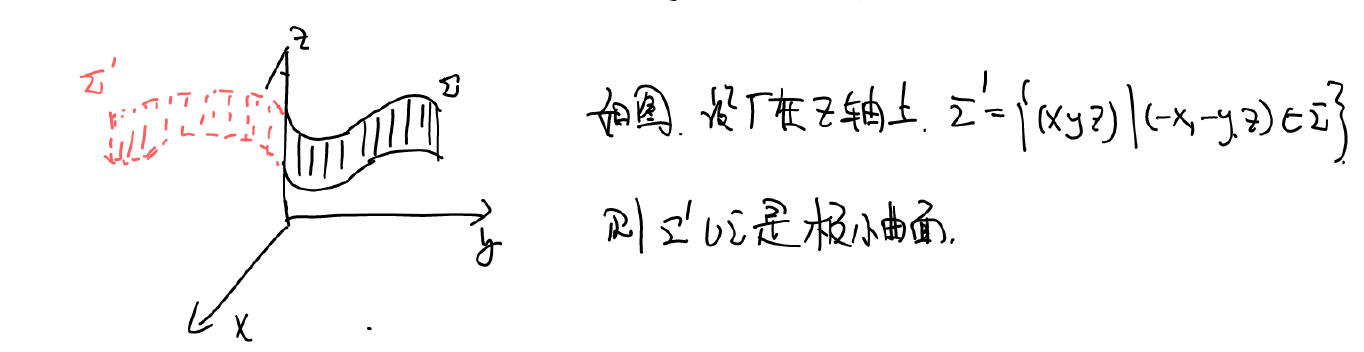
\includegraphics[scale=0.5]{images/reflection1.png}
	\caption{Schwartz反射}
	\label{reflection1}
\end{figure}

\begin{lemma}
    设$\mathbb{D}$为单位圆盘, $\mathbb{D}^+,\mathbb{D}^-$为上半/下半单位圆盘. 设$u: \mathbb{D}^+ \to \R$是调和函数, 且在$x-$轴上, $u\eq 0$. 在$\mathbb{D}$上定义
    \begin{equation}
        \tilde{u}(x,y)= \left\{
            \begin{aligned}
                &u(x,y), (x,y) \in \mathbb{D}^+.\\
                &-u(x,-y), (x,y) \in \mathbb{D}^-.
            \end{aligned}
        \right.
    \end{equation}
    则$\tilde{u}$是$\mathbb{D}$上的调和函数.
\end{lemma}
\begin{proof}
    显然, $\tilde{u}$连续且在$\mathbb{D}^+,\mathbb{D}^-$内部都是调和的, 我们只需要考虑$\tilde{u}$在$x-$轴附近的行为. $\forall x_0 \in x-axis$, 取$B_r(x_0) \subset \mathbb{D}$. 解方程
    \begin{equation}
        \left\{
            \begin{aligned}
                &\Delta v=0, x \in B_r\\
                & v|_{\partial B_r(x_0)}=0
            \end{aligned}
        \right.
    \end{equation}
    方程的可解性由Poisson积分给出,在复坐标$z=x+iy$下
    \begin{equation}
        v(a)=\frac{1}{2\pi} \int_{\abs{z-x_0}=r} \frac{r^2-\abs{a-x_0}^2}{\abs{z-a}^2}\tilde{u}(z)ds
    \end{equation}
    由于$\forall z \in \partial B_r(x_0), \tilde{u}(z)=-\tilde{u}(\bar{z})$. 则$\forall a\in B_r, v(a)=-v(\bar{a})$. 则在$x-$轴上, $v\eq 0$. 因此, $v|_{\partial{B_r^+}}=\tilde{u}|_{\partial{B_r^+}}$, $v|_{\partial{B_r^-}}=\tilde{u}|_{\partial{B_r^-}}$. 由最大值原理可知在$B_r$上, $\tilde{u}=v$. 因此, $\tilde{u}$是调和的.
\end{proof}
\begin{lemma}[等温坐标的存在性]
    设$(\M^2, g)$是二维黎曼流形, 则存在$\M^2$上的一组坐标卡$\{z=x+iy\}$, 使得在这组坐标下, $g=\lambda^2\abs{dz}^2=\lambda^2(dx^2+dy^2)$, 并且这组坐标下的坐标变换是全纯的.
\end{lemma}
\begin{proof}
    见附录.
\end{proof}
\begin{figure}[ht]
	\centering
	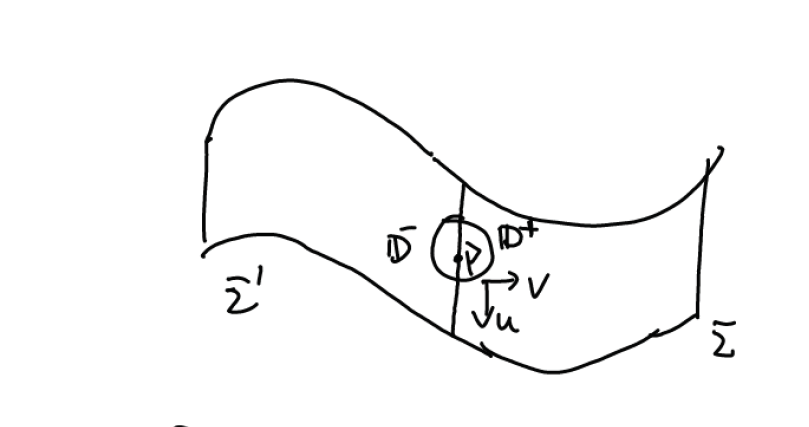
\includegraphics[scale=0.8]{images/reflection2.png}
	\caption{等温坐标}
	\label{reflection2}
\end{figure}
\begin{proof}[命题\eqref{min_reflection}的证明]
    取$\Sigma$上的等温坐标, 显然地, $\Sigma$上的等温坐标经反射后得到$\Sigma'$上的等温坐标. 将$z-$轴看作是$\mathbb{C}=\{w=u+iv\}$上的$u-$轴. 将$B_r(p)\cap \Sigma$看作 $\mathbb{D}^+$, 将$B_r(p) \cap \Sigma'$看作$\mathbb{D}^-$. 根据构造, 
    \begin{equation}
        x(w)=-x(\bar{w}), y(w)=-y(\bar{w})
    \end{equation}
    现在, 利用调和函数的反射性质可知, 在$\Sigma \cap \Sigma'$上, $x,y$坐标都是调和的. 我们只需要说明$z-$坐标也是调和的即可. 由$\Sigma'$的构造可知, 
    \begin{equation}
        z(u,v)=z(u,-v). 
    \end{equation}
    设$\vec{n}$是$B_r\cap \Sigma$在$z-$轴上的单位法向, 则$\frac{\partial z}{\vec{n}}= \partial_v{z}=0$. 于是, $z$满足 
    \begin{equation}
        \partial_v z(u,v)=-\partial_v z(u,-v). 
    \end{equation}
    由Schwzrtz 反射可知, $z_v$是调和函数, 则$z$是调和的. 
\end{proof}
\begin{remark}
    由此可见, 极小曲面上包含直线是非常强的条件. Schwartz反射的一类非常重要的应用是当极小曲面的边界上包含两条平行的直线的情况下.  这个时候我们可以做无穷多次反射得到一个周期的极小曲面.
\end{remark}
\begin{proposition} \label{conformal_im}
    设 $X(u,v): \mathbb{D} \to \R^3$是共形浸入. 则$\Sigma = X(\mathbb{D})$是极小曲面当且仅当$X$的每个分量是调和函数.
\end{proposition}
\begin{proof}
    由于$X$是共形浸入, 则在$\Sigma$上的度量在$z=u+iv$坐标下可以表示为$\lambda^2\abs{dz}^2$的形式, 而$\Delta_\Sigma X= \frac{1}{\lambda^2} \Delta X=0$.
\end{proof}
\begin{remark}
    $\Sigma\subset \R^3$是极小曲面当且仅当$\R^3$中的坐标函数在$\Sigma$上的限制是调和的, 这里$\Sigma$上必须是继承自$\R^3$上的度量. 命题 \eqref{conformal_im}中的共形浸入的条件是必不可少的, 比如, 设$X:\mathbb{D}\to \R^3, X(u,v)=(u,v,uv)$. 显然地, $\Delta X=0$. 但是$X(\mathbb{D})$不是极小曲面.
\end{remark}
\section{单调性公式}
\begin{proposition}[余面积公式]
    设$\Sigma^{n-1}\subset \R^n$是光滑曲面.  设$h: \Sigma \to \R$是Lipschitz, proper(紧集的原像为紧集)映射.  则$\forall f \in L^1_{\loc}(\Sigma)$, 成立
    \begin{equation}
        \int_{\{h < t\}} f \abs{\nabla_\Sigma h}d{\Haus}^{n-1}=\int^t_{-\infty} \int_{\{h=r\}}f d{\Haus}^{n-2}dr
    \end{equation}
\end{proposition}
余面积公式相当于Fubini定理, 可以将多重积分变为累次积分来计算. 例如, 取$\Sigma =\Omega, h(x,y)=x, f(x,y)=\chi_\Omega, t=+\infty$. 那么, 在余面积公式中, 
\begin{align}
    &\text{左侧}= \int_{\R^2}\chi_\Omega = \abs{\Omega}\\
    &\text{右侧}= \int^{+\infty}_{-\infty} \int_{\{x=r\}} \chi_\Omega dydr=\abs{\Omega}
\end{align}
\begin{proposition}
设$\Sigma^{n-1}\subset \R^n$是光滑曲面. 设$t>s$且$B_t(p) \cap \partial \Sigma =\emptyset$. 设$f \in C^1(\Sigma)$, $\vec{H}$是$\Sigma$的平均曲率向量.  则有    
\begin{equation}
    \begin{split}
        &\frac{1}{t^{n-1}}\int_{\Sigma\cap B_t} f d{\Haus}^{n-1}-\frac{1}{s^{n-1}}\int_{\Sigma\cap B_s} f d{\Haus}^{n-1} \\
        =& \int_{\Sigma \cap (B_t-B_s)} f \frac{\abs{(x-p)^\perp}^2}{\abs{x-p}^{n+1}} \\
        &+\frac{1}{2}\int^t_s \frac{1}{r^n}\int_{\Sigma\cap B_r}(r^2-\abs{x-p}^2)\Delta_{\Sigma}f+2f\inner{\vec{H}}{(x-p)^\perp}d{\Haus}^{n-1}dr
    \end{split}
\end{equation}
\end{proposition}
\begin{proof}
     记$I(r)=\frac{1}{r^{n-1}}\int_{\Sigma\cap B_r} f$. 不失一般性, 设$p=0$. 对$I(r)$求导,则有
     \begin{equation} \label{ddr}
        \ddr I(r)=-(n-1)\frac{1}{r^n}\int_{\Sigma \cap B_r} f + \frac{1}{r^{n-1}}\ddr \int_{\Sigma \cap B_r} f
     \end{equation}
     我们分别计算上式右侧的两项. 首先来计算第二项. 设$f=g\frac{\abs{x^T}}{\abs{x}}=g\abs{\nabla_\Sigma \abs{x}}$. 则由余面积公式(取$h=\abs{x}$),
     \begin{equation}
        \begin{split}
            \int_{\Sigma \cap B_r} f = \int_{\{\abs{x} < r\}\cap \Sigma }g \abs{\nabla_\Sigma \abs{x}} &= \int^r_{-\infty} \int_{\{\abs{x}=\rho\} \cap \Sigma} g d{\Haus}^{n-2}d\rho 
            %&= \int^r_{-\infty}\int_{\partial B_\rho \cap \Sigma} g
        \end{split}
     \end{equation}
     因此, 
     \begin{equation} \label{ddr2}
        \ddr \int_{\Sigma \cap B_r} f= \int_{\partial B_r \cap \Sigma} f \frac{\abs{x}}{\abs{x^T}} =r\int_{\partial B_r\cap \Sigma} f \frac{1}{\abs{x^T}}.
     \end{equation}
     设$\vec{n}$是$B_r\cap \Sigma$在$\partial B_r\cap \Sigma$上的单位法向. 容易验证 $\inner{x^T}{\vec{n}}= \abs{x^T}$.  现在,我们来计算第一项. 由$\Delta_\Sigma \abs{x}^2=2(n-1)+2\inner{\vec{H}}{x^\perp}$及分部积分公式可知,
     \begin{equation} \label{ddr1}
        \begin{split}
            2(n-1)\int_{\Sigma \cap B_r}f =&\int_{\Sigma \cap B_r}f \Delta_{\Sigma}\abs{x}^2-2\int_{\Sigma \cap B_r} f\inner{\vec{H}}{x^\perp} \\
            =& \int_{\Sigma \cap B_r}\abs{x}^2 \Delta_\Sigma f + 2\int_{\partial B_r\cap \Sigma}f\inner{\vec{n}}{x^T}  \\
            &- \int_{\partial B_r \cap \Sigma}\abs{x}^2 \inner{\vec{n}}{\nabla_{\Sigma}f}-2\int_{\Sigma \cap B_r} f\inner{\vec{H}}{x^\perp}\\
            &=I+II+III+IV
        \end{split}
     \end{equation}
     现在,在等式\eqref{ddr1}中,
     \begin{equation}
        II=2\int_{\partial B_r\cap \Sigma}f\abs{x^T}.
     \end{equation}
     \begin{equation}
        III=-r^2\int_{\partial B_r\cap \Sigma} \inner{\vec{n}}{\nabla_\Sigma f} =-r^2\int_{{B_r} \cap \Sigma} \Delta_{\Sigma}f.
     \end{equation}
     现在, 将\eqref{ddr1}及\eqref{ddr2}代入到\eqref{ddr}中, 则有
     \begin{equation}\label{ddr_i}
        \begin{split}
            \ddr I(r) =& -\frac{1}{2r^n}\int_{\Sigma \cap B_r}\abs{x}^2 \Delta_\Sigma f - \frac{1}{r^n} \int_{\partial B_r\cap \Sigma} f \abs{x^T} + \frac{1}{2r^{n-2}} \int_{B_r\cap \Sigma} \Delta_\Sigma f \\
            &+ \frac{1}{r^n} \int_{\Sigma \cap B_r fH\abs{x^\perp}} + \frac{1}{r^{n-2}} \int_{\partial B_r \cap \Sigma} \frac{f}{\abs{x^T}} \\
            =& \frac{1}{2r^n} \int_{\Sigma \cap B_r}(\Delta_\Sigma f(r^2-\abs{x}^2) + 2\inner{\vec{H}}{x^\perp}) + \frac{1}{r^n}\int_{\partial B_r\cap \Sigma} f \frac{\abs{x^\perp}^2}{\abs{x^T}}
        \end{split}
     \end{equation}
     再次利用余面积公式以及$\abs{\nabla^\Sigma\abs{x}}=\frac{\abs{x^T}}{\abs{x}}$, 上式右侧第二项的积分为
     \begin{equation} \label{ddr_i2}
        \begin{split}
            \int^t_s \frac{1}{r^n} \int_{\partial B_r \cap \Sigma} f \frac{\abs{x^\perp}^2}{\abs{x^T}^2} &= \int^t_s \int_{\{\abs{x} = r\}\cap \Sigma} f  \frac{\abs{x^\perp}^2}{\abs{x^T}} \frac{1}{\abs{x}^n} \\
            &= \int_{\{s<\abs{x}<t\}\cap \Sigma } f \frac{\abs{x^\perp}^2}{\abs{x^T}}\frac{1}{\abs{x}^n}\abs{\nabla_\Sigma\abs{x}} \\
            &=\int_{(B_t-B_s)\cap \Sigma} f \frac{\abs{x^\perp}^2}{\abs{x}^{n+1}}
        \end{split}
     \end{equation}
     在等式$\eqref{ddr_i}$两侧取积分, 并将\eqref{ddr_i2}代入即可得到单调性公式.
\end{proof}
\begin{corollary} \label{sub_harmonic}
    设$\Sigma^{n-1} \subset \R^n$是极小曲面. $x_0 \in \Sigma$, $B_s(x_0) \cap \partial \Sigma = \emptyset$. 设$f \in C^\infty(\Sigma)$且 $f \ge 0, \Delta_{\Sigma}f \ge -\frac{\lambda f}{s^2}$, 则有
    \begin{equation}
        f(x_0) \le e^{\frac{\lambda}{2}}\frac{\int_{B_s\cap \Sigma}f}{\abs{B_s\subset \R^{n-1}}}
    \end{equation}
\end{corollary}
\begin{proof}
    设$g(t)=\frac{1}{t^{n-1}}\int_{B_t\cap \Sigma}f, t\le s$.  将单调性公式代入$\frac{g(t+\Delta t)-g(t)}{\Delta t}$中并扔掉非负的部分, 求极限后得到
    \begin{equation}
        \begin{split}
            g'(t) &\ge \frac{1}{2}\frac{1}{t^n}\int_{B_t\cap \Sigma}(t^2-\abs{x}^2)\Delta_\Sigma f \\
            &\ge -\frac{\lambda}{2}\frac{1}{t^{n-2}s^2}\int_{B_t\cap \Sigma}f = -\frac{\lambda}{2}\frac{t}{s^2}g(t).
        \end{split}
    \end{equation}
    于是有,
    \begin{equation}
        \frac{g'(t)}{g(t)} \ge - \frac{\lambda}{2s^2}t\ge -\frac{\lambda}{2s}
    \end{equation}
    而这等价于: $\ddt (e^{\frac{\lambda t}{2s}}g(t)) \ge 0$. 因此, $\abs{B_1 \subset \R^{n-1}}f(x_0)=g(0) \le e^{\frac{\lambda}{2}}g(s)$, 证毕.
\end{proof}
\begin{corollary}
    设$\Sigma^{n-1} \subset \R^n$是极小曲面. $x_0 \in \R^n$, 设$f \in C^\infty(\Sigma)$且 $f \ge 0, \Delta_{\Sigma}f \ge 0$, 则
    \begin{equation}
        \frac{1}{s^{n-1}} \int_{B_s(x_0)\cap \Sigma}f
    \end{equation}
    关于变量$s$是非减函数. 特别地, 如果$x_0 \in \Sigma$, 那么对于任意$s>0$, 成立
    \begin{equation}
        f(x_0) \le \frac{\int_{B_s(x_0)\cap \Sigma} f}{ \abs{B_s\subset \R^{n-1}}}
    \end{equation}
\end{corollary}
\section{Gauss映射}
设$\Sigma \subset \R^3$是光滑曲面. 设$\vec{n}$为其单位法向. 由于在$\R^3$中, $\vec{n}$可以看作$\S^2$上的点, 我们可以得到映射$\N:\Sigma \to  \S^2, \N(p)=\vec{n}(p), p \in \Sigma$. 称$\N$为曲面 $\Sigma$的Gauss映射.
\begin{proposition}
    设$p \in \Sigma$, 则$T_{\N(p)}\S^2= T_p\Sigma$.
\end{proposition}
\begin{proof}
    $T_{\N(p)}\S^2=\{x\in \R^n\mid \inner{x}{\N(p)}=\inner{x}{\vec{n}}=0\}=T_p\Sigma$.
\end{proof}
回忆一下, $\II$表示标量值的第二基本形式, $\II(X,Y)=\inner{\nabla_XY}{\vec{n}}$, $\vec{n}$表示$\Sigma$的一个给定的单位法向. $\forall p \in \Sigma$, $\II$也可以看作是$T_p\Sigma \to T_p \Sigma$的线性映射.  $\forall X \in T_p\Sigma$, 定义$\II(X)$为唯一满足下列性质的向量$Z$.
\begin{equation}
    \forall Y \in T_p\Sigma, \inner{\II(X)}{Y}=\inner{Z}{Y}
\end{equation}
根据定义易知, $\II= \nabla \vec{n}$.
\begin{proposition}
    $\forall X, Y \in T_p\Sigma$, 有等式: 
    \begin{equation}
        \inner{\II(X,Y)}{\vec{n}}=-\inner{\nabla_X\vec{n}}{Y}=-\inner{d\N X}{Y}.
    \end{equation}
\end{proposition}
\begin{proof}
    由于$\inner{\vec{n}}{Y}=0$, 则有 $\inner{\nabla_XY}{\vec{n}}=-\inner{Y}{\nabla_X\vec{n}}$. 
    \par 第二个等式是因为 $\nabla_X\vec{n}=(\nabla \vec{n})X=d\N X$, 即是欧氏空间中的方向导数.
\end{proof}
\begin{proposition} \label{gauss_anticonformal}
    设$\Sigma \subset \R^3$是光滑曲面. 则$\Sigma$是极小曲面当且仅当其Gauss映射是反共形的($\S^2$上取由外单位法向所给定的定向). 反共形指的是保持角度大小而不保持方向.
\end{proposition}
\begin{remark}
    反向实际上排除了$\Sigma$是$\S^2$的一部分的情况.  
\end{remark}
\begin{proof}
    固定点$p \in \Sigma$. 由于$\II$是对称的, 则存在局部标架$\{e_i\}$, 使得在$p$点处, $\II e_1=\lambda_1 e_1$, $\II e_2=\lambda_2 e_2$. (这里, $\lambda_i,e_i$分别被称作曲面$\Sigma$的主曲率与主曲率方向). 现在,我们有
    \begin{equation}
        \inner{d\N e_i}{d\N e_j}= \inner{\nabla_{e_i}\vec{n}}{\nabla_{e_j}\vec{n}} =\lambda_i\lambda_j\inner{e_i}{e_j}
    \end{equation}
    显然地,  $dN=diag(\lambda_1,\lambda_2)$是反共形的当且仅当$\lambda_1+\lambda_2=0$, 当且仅当$\Sigma$是极小曲面.
\end{proof}
\begin{proposition}\label{pullback_gauss}
    设$\Sigma \subset \R^3$是极小曲面. $\N$为其Gauss映射. $d\Sigma, \omega$分别为$\Sigma, \S^2$上的面积形式, 设$N^*\omega$为其拉回. 则有
    \begin{equation}
        \abs{\II}^2d\Sigma= -2N^*\omega.
    \end{equation}
\end{proposition}
\begin{proof}
    如是同在命题\eqref{gauss_anticonformal}的证明中选择$\{e_i\}$. 设$\{e^{*i}\}$为其对偶标架. 由于$\lambda_1+\lambda_2=0$, 则
    \begin{equation}
        \abs{\II}^2d\Sigma=(\lambda_1^2+\lambda_2^2)e^{*1}\wedge e^{*2}=-2\lambda_1\lambda_2 e^{*1}\wedge e^{*2}.
    \end{equation}
    而由于$d\N=diag(\lambda_1,\lambda_2)$, 则 $\abs{\II}^2d\Sigma=-2N^* e^{*1} \wedge e^{*2}$.
\end{proof}
\section{Bernstein定理}
\begin{proposition} \label{caccio}
    设$u: \Omega \subset \R^2 \to \R$满足MSE. 设$\Sigma=\G(u)$. 设$\phi \in Lip(\Sigma)$且$\phi$具有紧支集, 则
    \begin{equation}
        \int_{\Sigma}\abs{\II}^2\phi^2 \le C\int_\Sigma \abs{\nabla_{\Sigma}\phi}^2
    \end{equation}
    这里,  $C$是万有常数.
\end{proposition}
\begin{proof}
    显然地, $\N(\Sigma) \subset \S^2_+$. 设$\omega$是 $\S^2$上的面积形式. 由于$\S^2_+$是单连通的, 则存在$1-$形式$\alpha$使得  $\Omega=d\alpha$. 而拉回与求微分是可交换的, 于是有 
    \begin{equation}
        \abs{\II}^2d\Sigma=-2\N^*\omega=-2\N^*d\alpha=-2d(\N*\alpha)
    \end{equation}
    由于$\forall 1-$形式$\beta$ , $d(\phi^2\beta)=\phi^2\beta+2\phi d\phi\wedge\beta$, 再由Stokes公式
    \begin{equation}
        \begin{split}
            \int_\Sigma \abs{\II}^2\phi^2 = -2 \int_\Sigma \phi^2 d(\N^*\alpha) &=-2\int_\Sigma d(\phi^2\N^*\alpha)+4\int_\Sigma \phi d\phi\wedge N^*\alpha\\
            &= 4\int_\Sigma  \phi d\phi\wedge N^*\alpha
        \end{split}
    \end{equation}
    在局部标架下, $\phi=\phi_i e^{*i}, N^*=diag(\lambda_1,\lambda_2), \alpha=\alpha_i e^{*i}$. 因此, 若设 $d\phi\wedge \N^*\alpha= f(x)d\Sigma$, 则 $\abs{f} \le C_\alpha \abs{\nabla_\Sigma \phi}\abs{\II}$. 于是有
    \begin{equation}
        \begin{split}
            \int_\Sigma \abs{\II}^2\phi^2 &\le C_\alpha \int_\Sigma \abs{\II}\abs{\phi} \abs{\nabla_\Sigma \phi} \\
            & \le C_\alpha(\epsilon \int_\Sigma \abs{\II}^2\phi^2 + \frac{1}{\epsilon}\int_\Sigma  \abs{\nabla_\Sigma \phi}^2 \\
        \end{split}
    \end{equation}
    取$\epsilon$使得 $\epsilon C_\alpha=\frac{1}{2}$即可.
\end{proof}
\begin{theorem}
    设$u: \R^2 \to \R$在全平面上满足MSE.  记$\Sigma=\G(u)$. 则$u$是仿射函数, 或者等价地, $\Sigma$是平面.
\end{theorem}
\begin{proof}
    我们首先说明, 如果下面的断言成立, 则$u$是仿射.
    \begin{claim*}
        $\forall k >0$,存在$\phi_k \in Lip(\Sigma)$使得  $\phi_k|_{B_k \cap \Sigma}=1$, $\phi_k$有紧支集 且$ \int_\Sigma \abs{\nabla_\Sigma \phi_k}^2 \to 0$.
    \end{claim*}
    若断言成立, 那么由不等式\eqref{caccio}可知, $\int_{\Sigma\cap B_k} \abs{\II}^2 \le \int_\Sigma \abs{\nabla_\Sigma \phi_k}^2 \to 0$. 则$\II\eq 0$. 因此$\Sigma$为平面. 
    \par 现在我们来证明断言成立. $\forall k>0$, 定义
    \begin{equation}
        \phi_k(x)=\left\{
            \begin{aligned}
                &1, \abs{x} < k, \\
                &1-\frac{\log\abs{x}-\log k}{\log k}, k \le \abs{x} \le k^2,\\
                &0, \abs{x} > k^2
            \end{aligned}
        \right.
    \end{equation}
    记$R_{s,t}=B_t-B_s$为环域. 将$R_{k,k^2}$分解为若干环域的并 
    \begin{equation}
        R_{k,k^2}=\cup_{i=0}^{\log k} R_{2^ik,2^{i+1}k}.
    \end{equation}
    直接计算可知, 在环域$R_{2^ik,2^{i+1}k}$上,
    \begin{equation}
        \abs{\nabla_\Sigma \phi} \le \abs{\nabla \phi} \le \frac{1}{\log k} \frac{1}{\abs{x}}
    \end{equation}
    以及
    \begin{equation} \label{logp}
        \abs{R_{2^ik,2^{i+1}k} \cap \Sigma } \le C 2^{2i}k^2. 
    \end{equation}
    上面的不等式其实
    于是,我们有
    \begin{equation}
        \int_\Sigma \abs{\nabla_\Sigma \phi_k}^2 \le C\sum_{i=0}^{\log k} 2^{2i}k^22\frac{1}{(\log k)^2} \frac{1}{2^{2i}k^2} \le C\frac{1}{\log k} \to 0.
    \end{equation}
    断言得证.
\end{proof}
下面我们提供一个Bernstein定理的非常初等的证明. 这个证明没有用到任何极小曲面方程的性质, 只用到了Gauss映射,球极投影和全纯函数的Liouville定理.
\begin{definition} \label{stereo}
    球极投影$\pi$是指$\S^2 \to \R^2$的的一个映射. 设$p \in \S^2$, 设$l$为经过点$p$与点$(0,0,1)$的直线. 设$l$与$xy$平面交于点$p'$, 定义$\pi(p)=p'$. 如图所示.
\end{definition}

\begin{figure}[ht]
	\centering
	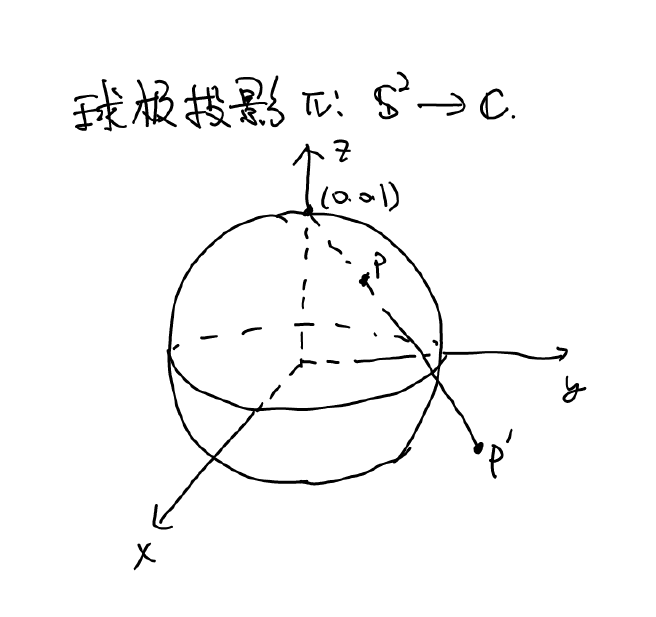
\includegraphics[scale=0.5]{images/stereo.png}
	\caption{球极投影}
	\label{stereopng}
\end{figure}
球极投影最重要的性质是它是共形(反共形,取决于我们选取的定向)映射, 这意味着我们可以将与$\S^2$有关的共形映射变为定义在 $\mathbb{C}$中某个区域上的亚纯函数. $\pi$与其逆的表达式为
\begin{align}
    &\pi(x,y,z)=(\frac{x}{1-z}, \frac{y}{1-z}), (x,y,z) \in \S^2\\
    &\pi^{-1}(w)= (\frac{2\Re w}{1+\abs{w}^2}, \frac{2\Im w}{1+\abs{w}^2}, \frac{-1+\abs{w}^2}{1+\abs{w}^2}), w \in \mathbb{C} \cup \{\infty\}.
\end{align}
\begin{proof}[Bernstein定理证明II]
    这里我们用设$f$满足极小曲面方程(字母$u$留作它用). 将散度形式展开后得到
    \begin{equation}
        (1+f_y^2)f_{xx}-2f_xf_yf_{xy}+(1+f_x^2)f_{yy}=0
    \end{equation}
    定义下列三个函数, 
    \begin{equation}
        a=\frac{1+f_x^2}{\sqrt{1+\abs{\nabla f}^2}},
        b=\frac{f_xf_y}{\sqrt{1+\abs{\nabla f}^2}},
        c=\frac{1+f_y^2}{\sqrt{1+\abs{\nabla f}^2}}
    \end{equation}
    由于$f$满足极小曲面方程, 直接计算可知: $a_y=b_x, b_y=c_x$.
    定义
    \begin{equation}
        \phi(x,y)=\int^x_0\int^y_0 b(s,t)dtds+\int^x_0\int^t_0a(s,0)dsdt+\int^y_0\int^t_0h(0,s)dsdt
    \end{equation}
    可知, 
    \begin{equation}
        \phi_{xx}=a, \phi_{xy}=b, \phi_{yy}=c.
    \end{equation}
    首先我们注意到, 
    \begin{equation}
        \det \nabla^2 \phi= ac-b^2 =1
    \end{equation}
    那么,  $\nabla^2 \phi$正定或者负定. 这里我们假设$\phi$为凸函数, 否则选取$-\phi$.  令
    \begin{equation}
        u=x+\phi_x, v=y+\phi_y.
    \end{equation}
    \begin{claim}
        $(u,v)$是 $\G(f)$上的等温坐标.
    \end{claim}
    显然地,由$\phi$的凸性可以知道, $(x,y)\to (u,v)$是$\R^2 \to \R^2$的微分同胚.  我们将$x,y$也看作是变量$(u,v)$的函数. 注意到, $\G(f)=\{(x,y,f(x,y))\mid (x,y) \in \R^2\}$. 在$(u,v)$坐标下则可以看作
    \begin{equation}
        \G(f)=\{(x(u,v), y(u,v), f(x(u,v), y(u,v)))\mid (u,v) \in \R^2\}.
    \end{equation}
    令$X(u,v)= (x(u,v), y(u,v), f(x(u,v), y(u,v)))$. 现在, 只需要证明$X$是共形嵌入即可. 即需要证明 $\inner{X_u}{X_v}=0$以及 $\abs{X_u}=\abs{X_v}$.
    \par 后面为了记号方便是, 记$p=f_x, q=f_y, w=\sqrt{1+f_x^2+f_y^2}$. 直接计算可知
    \begin{equation}
        \begin{bmatrix}
            &u_x &u_y \\
            &v_x &v_y
        \end{bmatrix}
        =
        \begin{bmatrix}
            &1+\frac{1+p^2}{w} & \frac{pq}{w} \\
            &\frac{pq}{w} & 1+\frac{1+q^2}{w}
        \end{bmatrix}
    \end{equation}
    那么, 
    \begin{equation}
        \begin{bmatrix}
            &x_u &x_v \\
            &y_u &y_v\\
        \end{bmatrix}
        =
        \frac{w}{(1+w)^2} 
        \begin{bmatrix}
            &1+\frac{1+q^2}{w} & -\frac{pq}{w} \\
            &-\frac{pq}{w} & 1+\frac{1+p^2}{w}
        \end{bmatrix}
    \end{equation}
    因此, 
    \begin{equation}
        \begin{split}
            X_u &=(x_u,y_u, f_xx_u+f_yy_u) \\
            &=\frac{w}{(1+w)^2}(1+w+q^2, -pq, p(1+w)).
        \end{split}
    \end{equation}
    \begin{equation}
        \begin{split}
            X_v &=(x_v,y_r, f_xx_v+f_yy_v) \\
            &=\frac{w}{(1+w)^2}(-pq, 1+w+p^2, q(1+w)).
        \end{split}
    \end{equation}
    这样, 断言得证. 现在, 我们知道当$\G(f)$赋予等温坐标后, 可以将$\G(f)$看作$\mathbb{C}$. 考虑Gauss映射$N$.  设$\pi$为球极投影. 我们知道$g=\pi\circ N \circ X$是共形的. 显然地, $N\circ X(\mathbb{C}) \subset \S^2_+$. 这样由球极投影的性质易知, $\abs{g} \ge 1$. 那么 $\abs{\frac{1}{g}} \le 1$. 而由于$\frac{1}{g}$是定义在$\mathbb{C}$上的全纯函数, 由Liouville定理可知, $g$常数. 即, $\G(f)$的Gauss映射为常值映射, 那么$\G(f)$必定为平面.
\end{proof}
\section{Weierstrass表示}
\begin{proposition} \label{iff_conformal}
    设$X: \Omega \to \R^3$光滑. $\Omega$上的坐标记为$(u,v)$. 则$X$是局部嵌入当然且当$dX$非退化. 并且, $X$是共形嵌入当且仅当$\abs{X_u}=\abs{X_v} \ne 0, \inner{X_u}{X_v} =0$.
\end{proposition}
\begin{proof}
    略.
\end{proof}
\begin{definition}
    设$\Omega \subset \R^2$.   $\Omega$上的坐标记为$(u,v)$, 复坐标记为$z=u+iv$. 对于任意$C^1$函数$f: \Omega \to \mathbb{C}$, 定义其形式偏导
    \begin{equation}
        \partial f= \frac{1}{2}(f_u- i f_v), \bar{\partial} f= \frac{1}{2}(f_u+i f_v).
    \end{equation}
    其它的记号$\partial_{z}f=\frac{\partial f}{\partial z} =\partial f$, $\partial_{\bar{z}}f=\frac{\partial f}{\partial \bar{z}} =\bar{\partial} f$也是常用的. 
\end{definition}
\begin{remark}
    易知, $\partial \barpartial f= \frac{1}{4}\Delta f$. 
\end{remark}
\begin{proposition} \label{iff_conformal_c}
    设$X: \Omega \to \R^3$是光滑嵌入. $X=(X_1,X_2,X_3)$. $\forall k$, 定义 $\phi_k= 2\partial X_k$. 则
    \begin{enumerate}
        \item $X$是共形的当且仅当$\sum_k \phi_k^2=0$.
        \item 若$X$是共形的, 则$X(\Omega)$是极小曲面当且仅当$\forall k, \phi_k$全纯.
        \item 若$X$是共形的, 则$X(\Omega)$上的度量可以表示为
        \begin{equation}
            ds^2=\frac{1}{2}\sum_k \abs{\phi_k}^2 \abs{dz}^2
        \end{equation}
    \end{enumerate}
\end{proposition}
\begin{proof}
    对于性质(1), 直接计算可知
    \begin{equation}
        \begin{split}
            (\frac{1}{2}\phi_k)^2=(\partial X_k)^2 &= \frac{1}{4}(\frac{\partial X_k}{\partial u} - i \frac{\partial X_k}{\partial v})^2\\
             &= \frac{1}{4}((\frac{\partial X_k}{\partial u})^2- (\frac{\partial X_k}{\partial v})^2) - \frac{1}{2}i \frac{\partial X_k}{\partial u} \frac{\partial X_k}{\partial v}
        \end{split}
    \end{equation}
    因此,  $\sum_k \phi_k^2= (\abs{X_u}^2- \abs{X_v}^2)-2i\inner{X_u}{X_v}$. 由命题\eqref{iff_conformal}可知结论成立.
    \par 对于性质(2), 我们知道$X(\Omega)$是极小的当且仅当$\forall k, X_k$是调和函数. 而
    \par $X_k$调和 $\iff$ $\barpartial \partial X_k=0$ $\iff$ $\partial X_k$全纯 $\iff$ $\phi_k$全纯.
    \par 性质(3)可由$ds^2=\abs{X_u}^2du^2+2\inner{X_u}{X_v}dudv+\abs{X_v}^2dv^2$及性质(2)得到.
\end{proof}
在单连通域上, 通过取$\Phi_k = \int \phi_k$, 我们可以得到以下定理:
\begin{theorem}[Weierstrass表示]
    任意极小曲面 $\Sigma$者可以局部地由三个满足 $\sum_k \Phi_k'^2=0$ 的全纯函数 $\Phi_k$ 确定, 并且$\Sigma$可以表示为 $\Sigma=X(\Omega)$, $X: \Omega \to \R^3$满足 
    \begin{equation}
        \begin{split}
            X &=\Re (\Phi_1,\Phi_2,\Phi_3) \\
             &=\Re \int^z (\phi_1,\phi_2,\phi_3)
        \end{split}
    \end{equation}
\end{theorem}
\begin{proof}
    我们已经证明了任意满足这样条件的三个全纯函数都可以确定一个极小曲面. 而等温坐标及调和共轭的存在性则保证了每个极小曲面都可以局部地表示成这样的形式.  $\forall p \in \Sigma$, 取$p$点处的等温坐标. 不失一般性, 可以假设$B_r \cap \Sigma= X(\mathbb{D})$, $X: \mathbb{D} \to \R^3$. 那么, $X$的三个分量都是调和函数. 而调和函数都可以作为全纯函数的实部,  因此存在三个全纯函数 $\Phi_k$使得  $X=\Re(\Phi_1,\Phi_2,\Phi_3)$.
\end{proof}
由该定理可以知道, 要构造一个极小曲面, 我们只需要构造三个全纯函数$\{\Phi_k\}$使得 $\sum \Phi_k'^2=0$即可. 给定全纯函数$f$及亚纯函数$g$, 取
\begin{equation}
    \phi_1=\frac{1}{2}f(1-g^2), \phi_2=\frac{i}{2} f(1+g^2), \phi_3=fg
\end{equation}
那么, $\sum_k \phi_k^2=0$恒成立. 只要我们先取$f,g$使得$\phi_k$都是全纯函数, 便能得到一个极小曲面. 另一方面, 简单计算可知, 
\begin{equation}
    f=\phi_1-i\phi_2, g=\frac{\phi_3}{\phi_1-i\phi_2}= -\frac{\phi_1+i\phi_2}{\phi_3}
\end{equation}
因此, 每个极小曲面都可以局部地由 $(g,f)$给出. 称$(g,f)$为极小曲面的Weierstrass表示对. 
\begin{remark}
    为了使得$\phi_k$都是全纯函数, 对于亚纯函数$g$的极点需要有一定的限制. 比如如果$f$在$p$点处有一个$n$阶零点, 那么$g$在$p$点处极点的阶数至多为$\frac{n}{2}$. 另外, 由于$X$是嵌入, $f$不包含零点.
\end{remark}
亚纯函数$g$实际上是Gauss映射, 下面的命题\eqref{g=gauss}阐述了这件事.  首先证明全纯函数的一个简单性质.
\begin{lemma}
    设$z=u+iv$, $F(z)=f(z)+ig(z)$, $f,g$均为实值函数. 那么
    \begin{enumerate}
        \item $\partial_u f = \Re F'$.
        \item $\partial_v f = -\Im F' $.
    \end{enumerate}
\end{lemma}
\begin{proof}
    直接代入定义及Cauchy方程即可.
    \begin{equation}
        \begin{split}
            F'=\partial F & = \frac{1}{2}(F_u-iF_v) \\
             &= \frac{1}{2}(f_u+ig_u-if_v+g_v) \\
             &= f_u-if_v
        \end{split}
    \end{equation}
\end{proof}
\begin{proposition} \label{g=gauss}
    设$\Omega$为单连通区域.  $X: \Omega \to \R^3$为共形嵌入且 $X(\Omega)$为极小曲面. 设$\pi: \S^2 \to \mathbb{C}$是球极投影. $N$为$X(\Omega)$的Gauss映射. 设$(g,f)$为$X$的Weierstrass表示对. 则
    \begin{align}
        &ds^2=\lambda^2\abs{dz}^2=\frac{1}{4}\abs{f}^2(1+\abs{g}^2)^2\abs{dz}^2.  \label{fg_metric}\\
        &g=\pi\circ N  \circ X.
    \end{align}
\end{proposition}
\begin{proof}
    $ds^2$可直接计算. 对于Gauss映射, 首先 由全纯函数的性质可知, 
    \begin{align}
        &\partial_u \Re \int \phi= \Re \phi \\
        &\partial_v \Re \int \phi= -\Im \phi
    \end{align}
    因此,我们有
    \begin{equation}
        \begin{split}
            &X_u \wedge X_v  \\
            =&-(\Re \phi_1,\Re \phi_2, \Re \phi_3) \wedge (\Im \phi_1, \Im \phi_2, \Im \phi_3) \\
            =&- \begin{bmatrix}
                &\Re \phi_1 & \Re \phi_2 &\Re \phi_3 \\
                &\Im \phi_1 & \Im \phi_2 &\Im \phi_3 \\
                &\partial_1 & \partial_2 &\partial_3
            \end{bmatrix} \\
            =&-(\Re\phi_2 \Im \phi_3- \Im \phi_2 \Re \phi_3, \Re \phi_3 \Im \phi_1- \Im\phi_3 \Re \phi_1, \Re \phi_1 \Im \phi_2 - \Re\phi_2 \Im \phi_3) \\
            =&(\Im \phi_2 \bar{\phi}_3, \Im \phi_3 \bar{\phi}_1, \Im \phi_1 \bar{\phi}_2) \\
            =&(\Im \frac{i}{2}\abs{f}^2(1+g^2)\bar{g}, \frac{1}{2}\abs{f}^2(1-\bar{g}^2)g, \Im \frac{i}{4}\abs{f}^2(1-g^2)(1-\bar{g}^2)) \\
            %=& \frac{1}{4}(2\lambda^2\Re g, 2\lambda^2 \Im g, \lambda^2(\abs{g}^2-1))
        \end{split}
    \end{equation}
    这里, $\Re, \Im$分别表示实部与虚部. 于是, 
    \begin{equation}
        \abs{X_u \wedge X_v}=\frac{1}{4}\abs{f}^2(1+\abs{g}^2)^2
    \end{equation}
    \begin{equation}
        N=\frac{X_u\wedge X_v}{\abs{X_u\wedge X_v}}= \frac{1}{1+\abs{g}^2}(2\Re g, 2 \Im g, \abs{g}^2-1)
    \end{equation}
    最终由球极投影的定义\eqref{stereo}可知 $\pi\circ N \circ X=g$.
\end{proof}
由上面的命题可知, 亚纯函数$g$的极点的几何含意是明显的, 在$g$的极点处, 极小曲面的单位法向垂直向上.
\par 另一种表示方法为$(g,dh)$. 这里$g$如上. $dh$为亚纯微分. 我们只需要取$dh=fgdz$即可.这样, Weierstrass表示也可以写为
\begin{equation}
    X=\Re \int^z (\frac{1-g^2}{2g}, \frac{i(1+g^2)}{2g},1)dh
\end{equation}
在这种表示下, $dh$被称为高度微分(height differential), 它的几何含意也是明显地, 我们有
\begin{equation}
    \Re dh= dX_3.
\end{equation}
\subsubsection{极小曲面的例子}
Catenoid: $g(z)=z, dh=\frac{1}{z}dz, z \in \mathbb{C}-\{0\}$.  
\par Catenoid是由悬链线($xz$平面上的曲线$x=\cosh z$)旋转而得到的.

\begin{figure}[ht]
	\centering
	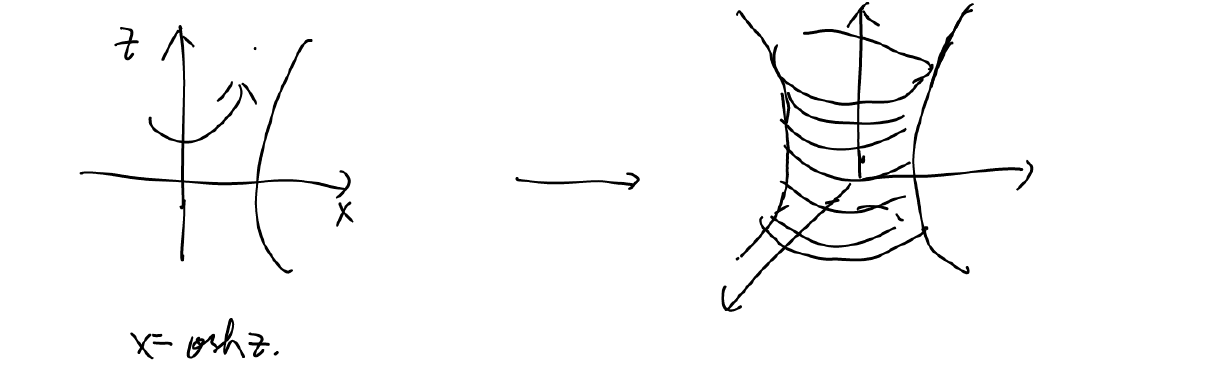
\includegraphics[scale=0.5]{images/catenoid.png}
	\caption{Catenoid}
	\label{catenoidp}
\end{figure}


Helicold: $g(z)=z, dh= \frac{i}{z}, z \in \mathbb{C}-\{0\}$.
Helicold是由一条水平直线匀速螺旋上升而得到的. Helicold可以局部地表示为$z=\arctan\frac{y}{x}$的形式.

\begin{figure}[ht]
	\centering
	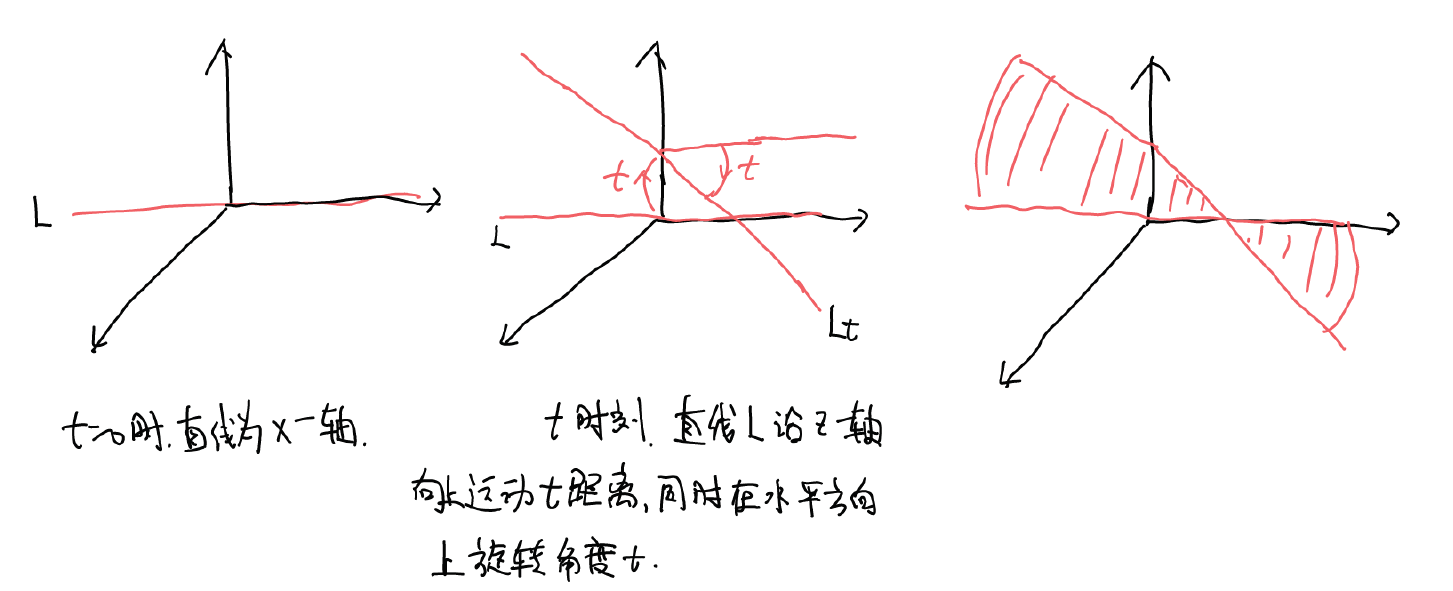
\includegraphics[scale=0.5]{images/helicoid.png}
	\caption{Helicoid}
	\label{helicoidp}
\end{figure}
\par Catenoid与Helicold的关系: Helicold可以由Catenoid连续变化而得到. 注意观察它们的Weierstrass表示对分别为$(z,\frac{1}{z}dz)$, $(z,\frac{i}{z}dz)$.
\begin{align}
    &\text{Catenoid}= \Re \int (\frac{1-z^2}{2z}, \frac{i(1+z^2)}{2z},1)\frac{1}{z}dz \\
    &\text{Helicold}= \Re i \int (\frac{1-z^2}{2z}, \frac{i(1+z^2)}{2z},1)\frac{1}{z}dz \\
\end{align}
现在, 定义
\begin{equation}
    \Sigma_t= \Re e^{\frac{\pi it}{2}} \int (\frac{1-g^2}{2g}, \frac{i(1+g^2)}{2g},1)\frac{1}{z}dz 
\end{equation}
\begin{figure}[ht]
        \center
        \scriptsize
        \begin{tabular}{cc}
                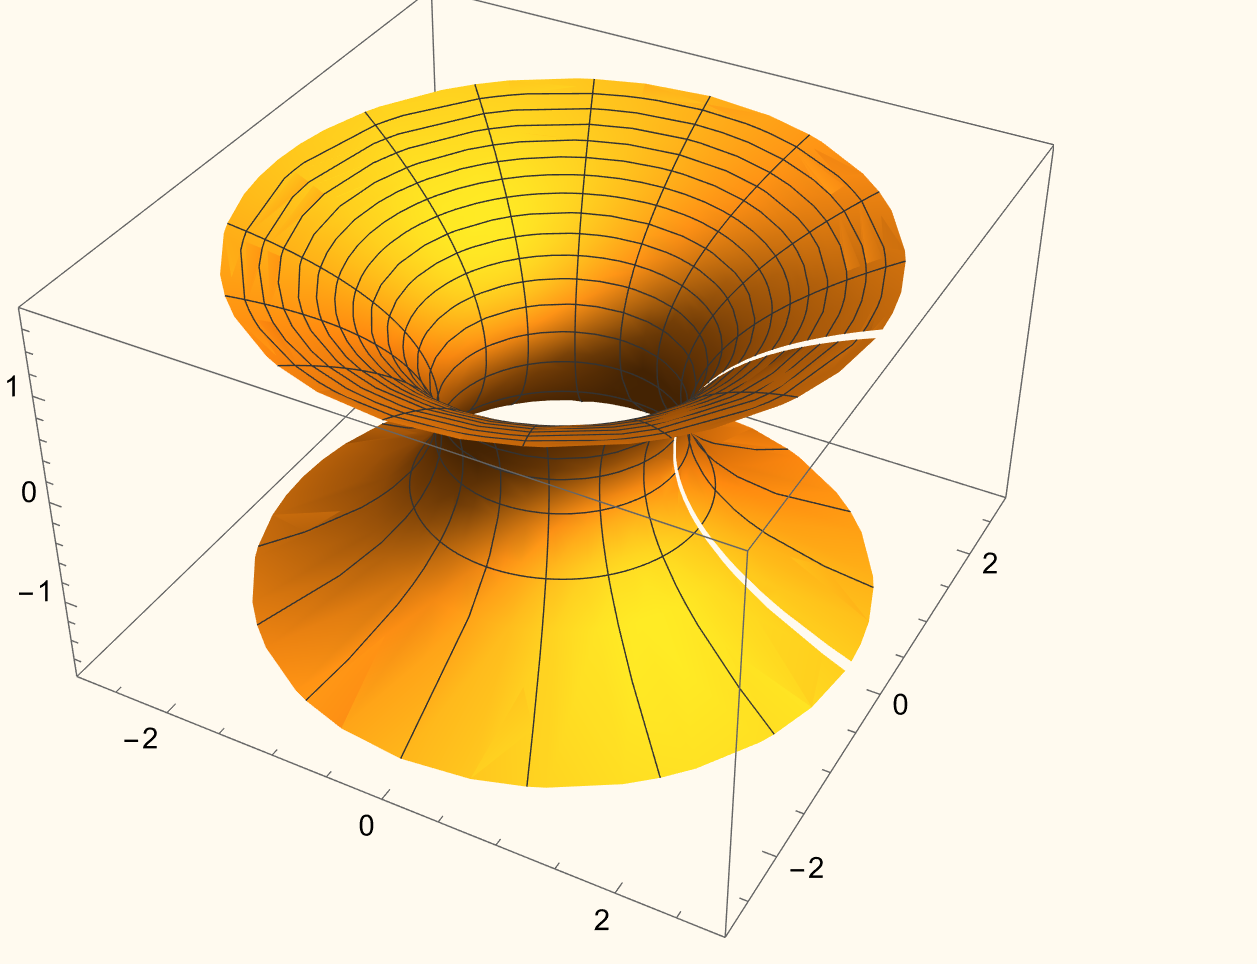
\includegraphics[scale=0.2]{images/catenoid2helicold0.png} &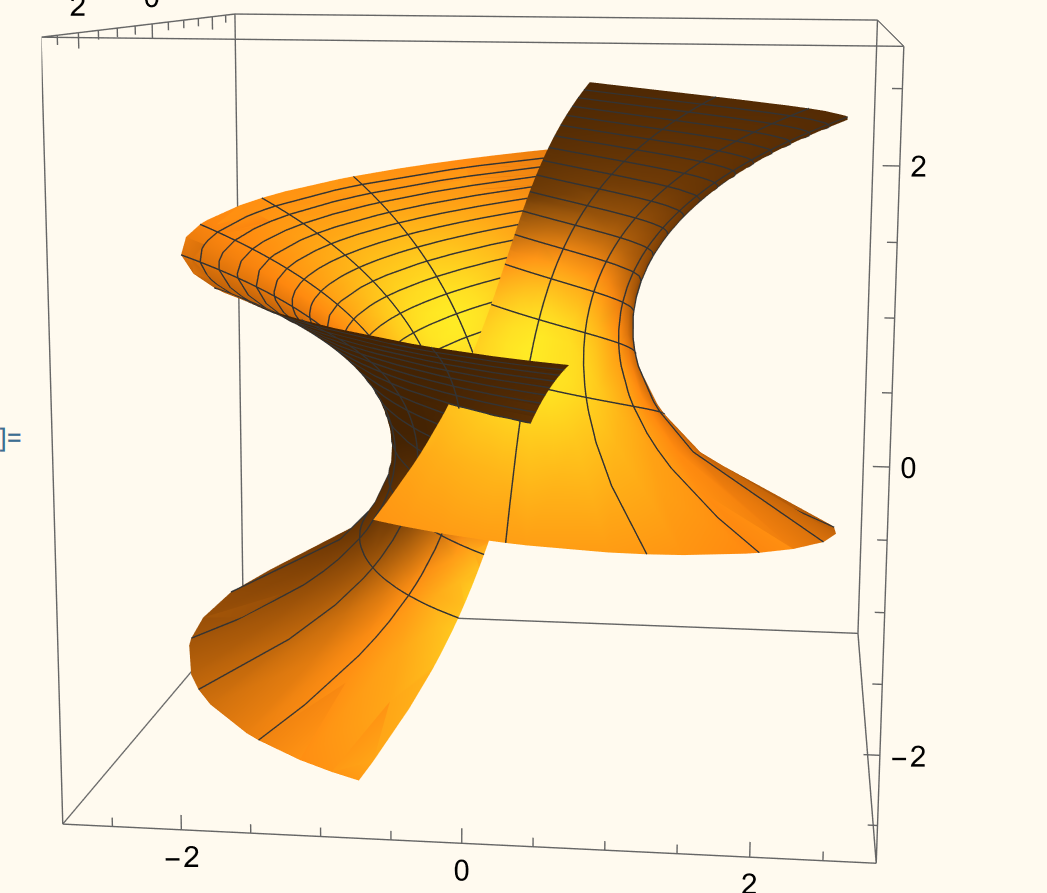
\includegraphics[scale=0.2]{images/catenoid2helicold1_10.png}\\
                ($t=0$) & ($t=\frac{1}{10}$) \\
                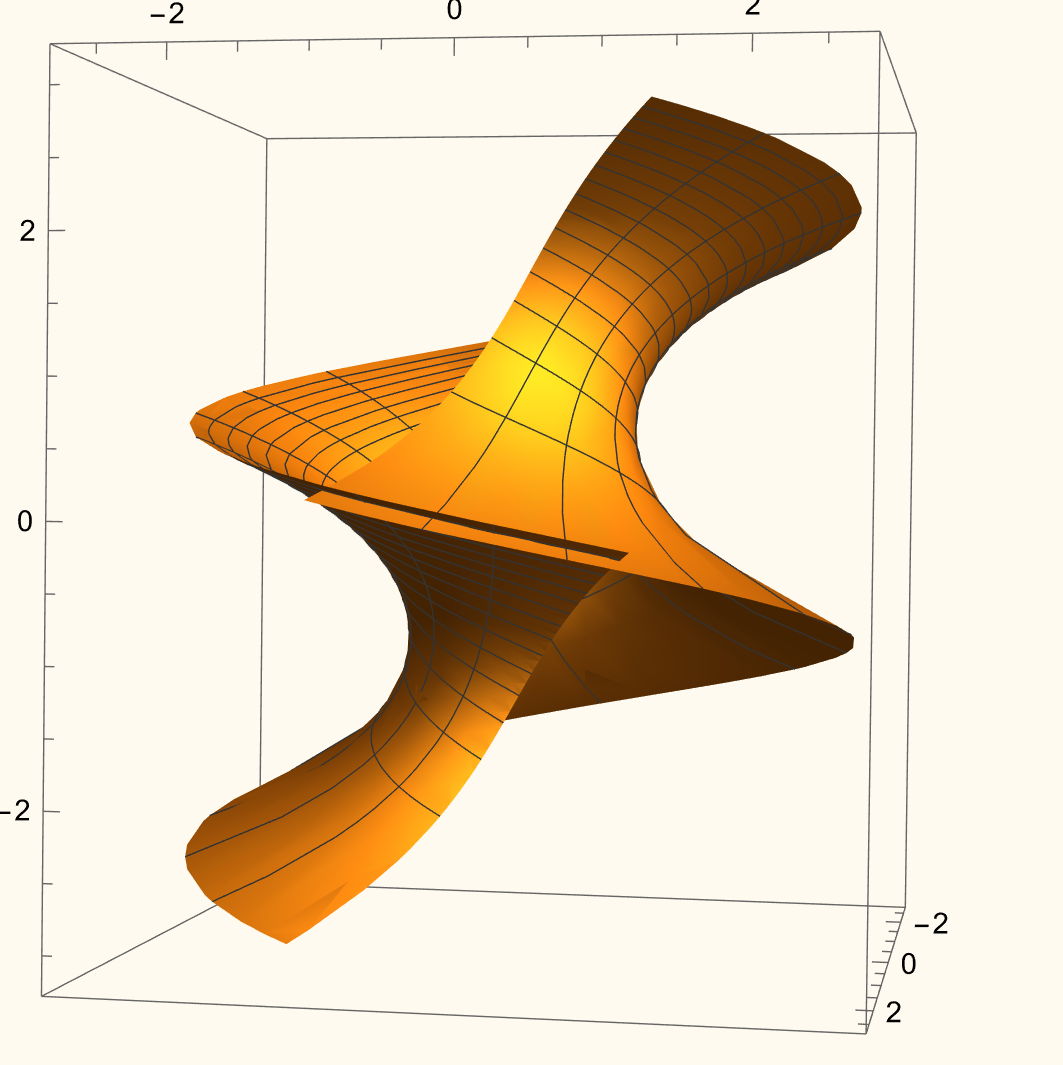
\includegraphics[scale=0.2]{images/catenoid2helicold1_3.png}& 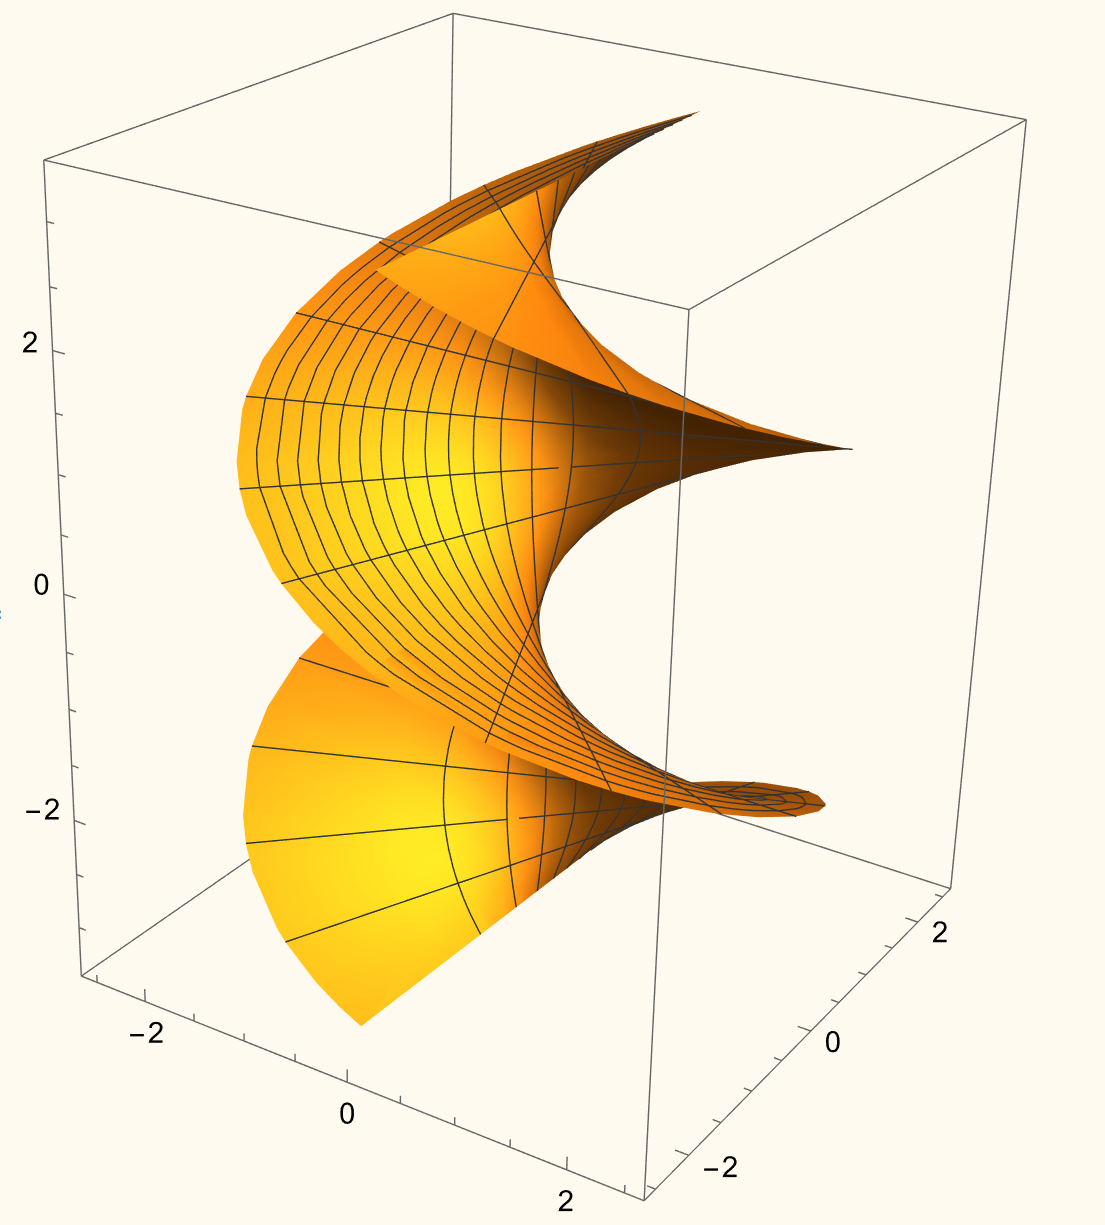
\includegraphics[scale=0.2]{images/catenoid2helicold1.png}\\
                ($t=\frac{1}{3}$) & ($t=1$) \\
        \end{tabular}
        \caption{Catenoid到Helicoid的连续形变}
        \label{catenoid2helicoid}
        %\vspace{-0.5em}
\end{figure}
那么, 对于每一个$\theta$, $\Sigma_\theta$都是极小曲面, 并且$\theta=0,1$时得到的分别为Catenoid与Helicoid.  图\eqref{catenoid2helicoid}表示了这个连续变化的过程.
\par The singly periodic Scherk surface.  单周期Scherk surface的Weierstrass表示为
\begin{equation*}
    g(z)=z, dh=\frac{iz}{z^4-1}
\end{equation*}
\begin{equation*}
    X(z)=\Re \int^z_0(\frac{1}{2}\frac{1-w^2}{w}, \frac{i}{2}\frac{1+w^2}{w},1)\frac{iw}{w^4-1}dw
\end{equation*}
这里, $\int^z_0$表示沿条连接$0$与$z$点的路径的曲线积分. 然而由于被积函数不是全纯的, 这个路径是依赖于路径的选取的.  我们接下来将会说明, 对路径的依赖将会导致\textbf{曲面具有周期性}.
\par 首先来看$X(z)$的$x$分量. 我们计算一下$x(z)$对路径的依赖是什么样的.  对于$x$坐标, $\{\pm i\}$是积分的奇点. 设$\alpha$, $\beta$为如图所示的两条路径, 那么
\begin{figure}[ht]
    \centering
    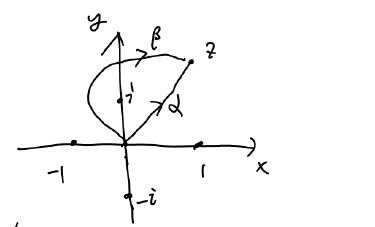
\includegraphics[scale=0.8]{images/scherk_x.png}
    \caption{x-coordinate}
    \label{scherk_x}
\end{figure}
\begin{equation}
    \begin{split}
        \int_{\alpha- \beta} \frac{1}{2}\frac{1-w^2}{w} \frac{iw}{w^4-1} &= -\frac{i}{2}\int_{\alpha-\beta} \frac{1}{1+w^2} \\
        &=-\frac{i}{2}2\pi i \Res(\frac{1}{1+w^2})\mid_{w=i} =-\frac{\pi}{2}i.
    \end{split}
\end{equation}
对于点$-i$处的计算也是如此. 因此, $x-$坐标与积分路径的选择无关. 同样地,对于$y-$坐标, $\{\pm 1\}$是其奇点. 设$\alpha, \beta$如图, 那么直接计算可知
\begin{figure}[ht]
    \centering
    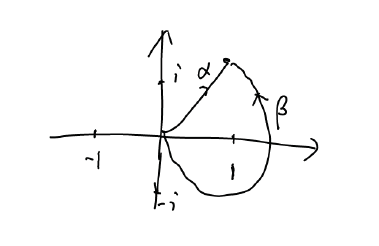
\includegraphics[scale=0.8]{images/scherk_y.png}
    \caption{y-coordinate}
    \label{scherk_y}
\end{figure}
\begin{equation}
    \begin{split}
        \int_{\alpha-\beta} \frac{i}{2}\frac{1+w^2}{w} \frac{iw}{w^4-1} &= \frac{1}{2}\int_{\alpha-\beta \frac{1}{1-w^2}} \\
        &= \frac{1}{2} 2\pi i \Res(\frac{1}{1-w^2} ) \mid_{w=1}=\frac{\pi}{2}i
    \end{split}
\end{equation}
因此, $y-$坐标也与路径的选择无关.  
\par 而对于$z-$坐标, 我们只以图\eqref{scherk_x}中的情况为例来说明.
\begin{equation}
    \int_{\alpha-\beta} \frac{iw}{w^4-1} = i 2\pi i \Res(\frac{w}{w^4-1}) \mid_{w=i} = \frac{\pi}{2}
\end{equation}
因此, $z-$坐标是路径的选择有关的. 令
\begin{equation}
    \Omega= \mathbb{C}-\{(x,y)\mid y=0, \abs{x}\ge 1 \text{ 或 } x=0, \abs{y}\ge 1\}
\end{equation}
那么, $\Omega$是单连通的. $\forall z \in \Omega$, 选择曲线$\alpha \subset \Omega$使得$\alpha(0)=0, \alpha(1)=z$. 那么我们就可以定义
\begin{equation}
    X(z)=\Re \int_{\alpha}(\frac{1}{2}\frac{1-w^2}{w}, \frac{i}{2}\frac{1+w^2}{w},1)\frac{iw}{w^4-1}dw
\end{equation}
由于我们选择了$\Omega$单连通, 那么$X$是良好定义的. 这样我们得到了$\Omega \to \R^3$的一个极小曲面.
\par $\forall z$, 选择$\beta$使得$\beta(0)=0, \beta(1)=z$, 但是比起$\alpha$, 我们要求$\beta$在点$i$处绕了一圈. 如图\eqref{scherk_z}所示.
\begin{figure}[ht]
    \centering
    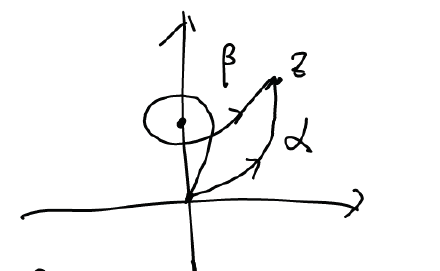
\includegraphics[scale=0.8]{images/scherk_3.png}
    \caption{z-coordinate}
    \label{scherk_z}
\end{figure}
定义
\begin{equation}
    \tilde{X}(z)=\Re \int_{\beta}(\frac{1}{2}\frac{1-w^2}{w}, \frac{i}{2}\frac{1+w^2}{w},1)\frac{iw}{w^4-1}dw
\end{equation}
\begin{figure}[ht]
    \centering
    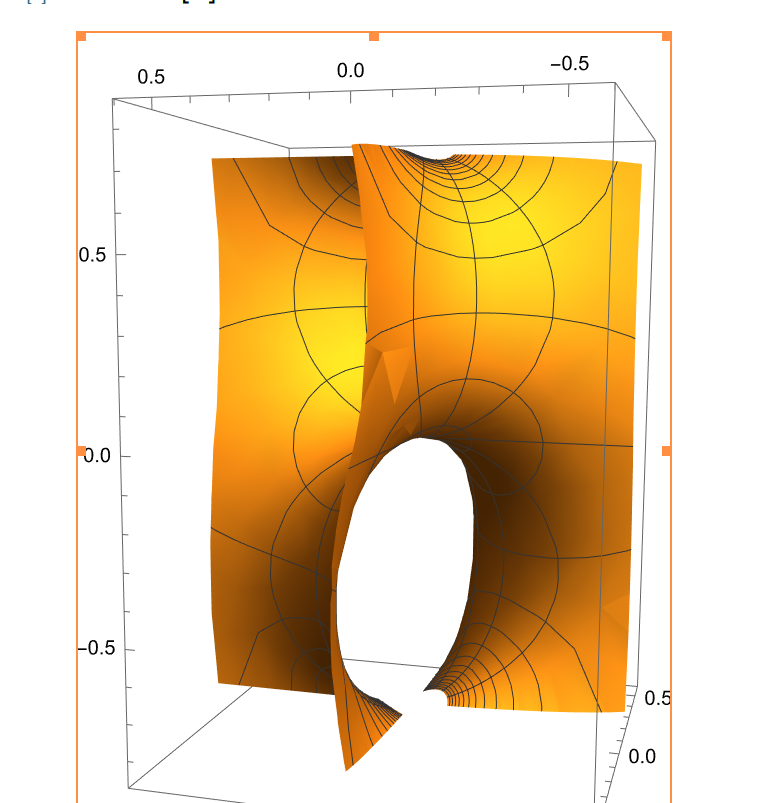
\includegraphics[scale=0.5]{images/scherkI.png}
    \caption{单周期Scherk曲面}
    \label{scherkI}
\end{figure}
根据我们之前的计算, $x=\tilde{x}, y=\tilde{y}, z=\tilde{z}-\frac{\pi}{2}$. 因此, $\tilde{X}(\Omega)$是$X(\Omega)$向上平移而得到的. 实际上, $X(\Omega)\cup \tilde{X}(\Omega)$可以光滑地拼接在一起. 另外, 假如我们选择$\beta$在点$i$处绕$k$圈时, 将恰好得到由$X(\Omega)$向上平移$\frac{k\pi}{2}$ 而得到的极小曲面. 将无数个这样的曲面拼接在一起就得到了单周期的Scherk surface. 图\eqref{scherkI}显示了Scherk曲面在一个周期内的图像(Helicoid也是同样的, 在$z-$方向上是周期的, 只是Helicoid时的周期性很容易得到).

借助于Weierstrass表示, 我们来研究Gauss映射的值分布, 并给出Bernstein定理的一个新的证明.
\begin{lemma} \label{nonzero_noncomplete}
    设$q$是$\mathbb{D}$上的全纯函数. 如果$q$没有零点, 那么度量$\abs{q}^2\abs{dz}^2$不是完备的.
\end{lemma}
\begin{proof}
    直接计算可知, 若$q$没有零点, 则$\abs{q}^2\abs{dz}^2$是平坦度量. 如果这个度量是完备的, 那么指数映射将给出$\mathbb{D}\to \mathbb{C}$的共形映射, 这是不可能的.
\end{proof}
\begin{theorem}
    设$\Sigma \subset\R^3$是非平坦的完备极小曲面, 则其Gauss映射的像在$\S^2$中稠密.
\end{theorem}
\begin{proof}
    设$\Sigma$是单连通的, 否则可以取$\Sigma$的万有覆盖. 如果$N(\Sigma)$不是稠密的, 可以旋转$\Sigma$, 使得$\overline{N(\Sigma)}$取不到$(0,0,-1)$的邻域.  这样得到的Gauss映射$\pi \circ g: \Sigma \to \mathbb{C}$是有界的, 即有$\abs{g} \le C$.  由于$\Sigma$是单连通的, 则$\Sigma$共形等价于 $\mathbb{D}$或者$\mathbb{C}$. 如果是前者, 则由等式\eqref{fg_metric}可知, $\Sigma$上的度量满足$ds^2 \le C\abs{f}^2\abs{dz}^2$. 由引理\eqref{nonzero_noncomplete}可知, $ds^2$不可能是完备的. 而如果是后者, 则得到了$\mathbb{C} \to \mathbb{C}$上的有界全纯函数$g$, 而此时$g$必定为常数,这意味着$\Sigma$是平坦的.
\end{proof}
\begin{corollary}
    如果$\Sigma \subset \R^3$是极小曲面, 且其Gauss映射的像不包含$\mathbb{S}^2$中的某个开集. 则$\Sigma$是平坦的.
\end{corollary}
\section{MSE revisited}
\begin{proposition}
    设$u,v$满足极小曲面方程, 则$w=u-v$满足一个线性椭圆方程
    \begin{equation}
        \div(a^{ij}w_i\PJ) =0
    \end{equation}
    并且存在常数$C=C(Du,Dv)$ 使得 $\frac{1}{C} \le \lambda_{\min} \le \lambda_{\max} \le C$.
\end{proposition}
\begin{proof}
    设$F: \R^n \to \R^n$, $F(x)=\frac{x}{\sqrt{1+\abs{x}^2}}$. 由微积分基本定理
    \begin{equation}
        \begin{split}
            F(Du)-F(Dv)= & \int^1_0 \ddt f(tDu+(1-t)Dv)dt \\
            =& \int^1_0 dF(tDu+(1-t)Dv)(Du-Dv)dt\\
            =& \int^1_0 dF(tDu+(1-t)Dv)dwdt\\
            =& a^{ij}w_i\PJ
        \end{split} 
    \end{equation}
    其中, $a^{ij}=\int^1_0 \frac{\partial F^i}{\partial x^j}(tDu+(1-t)Dv)dt$. \\
    由于$\div(F(Du)) = \div(F(Dv))=0$, 则
    \begin{equation}
        \div(a^{ij}w_i\PJ)=0.
    \end{equation}
    直接计算可知
    \begin{equation}
        \left[\frac{\partial F^i}{\partial x^j}\right] = \frac{1}{(1+\abs{x}^2)^\frac{3}{2}}((1+\abs{x}^2)I-xx^T)
    \end{equation}
    显然为正定矩阵, 且其特征为为 $\lambda_1=\frac{1}{(1+\abs{x}^2)^{\frac{3}{2}}}, \lambda_2=\cdots\lambda_n=\frac{1}{\sqrt{1+\abs{x}^2}}$. 结论得证.
\end{proof}
\begin{corollary}
    设$u,v$满足MSE, $u(p)=v(p)$且在$p$点的邻域内, $u \ge v$. 则 $u\eq v$.
\end{corollary}
\begin{proof}
    设$w=u-v$. 则在点$p$的邻域内, $w(p)=0$并且 $w \ge 0$. 由强最大值原理可知, $w\eq 0$.
\end{proof}
\begin{corollary}
    设$\Sigma_1,\Sigma_2 \subset \R^n$是极小曲面, 设$p \in \Sigma_1 \cap \Sigma_2$是$\Sigma_1,\Sigma_2$的内点. 若$\Sigma_1$ 完全位于$\Sigma_2$的同一侧, 则$\Sigma_1=\Sigma_2$.
\end{corollary}
\begin{proof}
    由假设条件, $\Sigma_1,\Sigma_2$在 $p$点处相切. 设$p$点的邻域中, $\Sigma_1=\G(u)$, $\Sigma_2=\G(v)$. 由于$\Sigma_1$完全位于$\Sigma_2$的同一侧, 这里不妨设为上方, 则$u \ge v$. 又由于$u(p)=v(p)$, 则由强最大值原理可知  $u \eq v$.
\end{proof}
\begin{theorem}
    设$\Omega \subset \R^2$是严格凸的. $\Gamma =\G(\psi) \subset \partial \Omega \times \R$, 其中, $\psi \subset C(\partial \Omega)$. 设$\Sigma \subset \R^3$是以$\Gamma$为边界的极小曲面, 则存在函数$u$使得 $\Sigma=\G(u)$.
\end{theorem}
\begin{proof}
    首先说明$\Sigma \subset \overline{\Omega} \times \R$. 否则, 取$x \in \Omega$, 取$R>0$使得$\Sigma \subset B_R\times \R$并且 $\Sigma$与$\partial B_R\times \R$相切于点$y \in \partial B_R \times \R$. 设$\tilde{\Sigma}$为$\partial B_R \times \R$ 在点$y$处的切平面, 则$\Sigma$完全位于$\tilde{\Sigma}$的同一侧且它们相切于点$y$. 由最大值原理可知, $\Sigma= \tilde{\Sigma}$, 这样便推出一个矛盾. 因此, $\Sigma \subset \overline{\Omega}\times \R$.
    \par 设$P_t$为平面$\{x_3=t\}$. 设$P_t$与$\Sigma$相交. 记$\Sigma_t^+$为$\Sigma$在平面$P_t$上侧的部分, $\Sigma_t^-$为$\Sigma$在平面$P_t$下侧的部分. 将$\Sigma_t^+$反射到$P_t$下侧, 记为$\tilde{\Sigma}_t^+$.  现在我们考虑下面两种情况:
    \begin{enumerate}
        \item  $\forall t$, $\tilde{\Sigma}_t^+\cap \Sigma_t^-=\emptyset$, 则$\pi:\Sigma\to \Omega$必定为单射. 否则, 若存在$p_1,p_2 \in \Sigma$使得 $\pi(p_1)=\pi(p_2)$, 不妨设$p_1$在上侧. 则取$t=\frac{1}{2}(z(p_1)+z(p_2))$时, 必定有$p_2 \in \tilde{\Sigma}_t^+\cap \Sigma_t^-$,  这样也假设矛盾. 因此, $\Sigma$ 作为某个函数的图像.
        \item $\exists t$使得 $\tilde{\Sigma}_t^+ \cap \Sigma_t^-\ne \emptyset$.  取这样最大的$t$. 则$\tilde{\Sigma}_t^+$完全位于$\Sigma_t^-$的上侧.  当$t$再减小时, 设$\Lambda=  \tilde{\Sigma}_t^+ \cap \Sigma_t^-$, 则$\Lambda \subset \Omega \times \R$(因为$\partial \Sigma$是边界上的$\G$, 因此$\Lambda$不可能与$\partial \Omega \times \R$相交). 显然地, $\Lambda$ 同时围出$\tilde{\Sigma}_t^+, \Sigma_t^-$上的两个极小曲面. 通过选取$t$足够接近$t_0$, 我们可以假设这两个极小曲面都能(旋转坐标系之后)写成函数的图像的形式, 这样便与最大值原理矛盾.
    \end{enumerate}
\end{proof}
\begin{remark}
    上面的定理将$\Sigma$写成函数$u$的图像之后, 虽然$\Sigma$是光滑的, 但是到现在为止我们还不能得到$u$的光滑性.
\end{remark}
\begin{theorem}
    设$u$满足MSE, 则$u$是实解析的.
\end{theorem}
\begin{proof}
    $n=2$时, \cite[p.125]{Nit1}中提供了一个非常简单的证明. 一般情况下请参考\cite{Giu84}及其中的参考文献.
\end{proof}
\begin{theorem}
    设$\Sigma_1,\Sigma_2 \subset \R^3$是极小曲面, 且$\Sigma_1,\Sigma_2$在点$p\subset \R^3$处相切. 则在$p$点的某个邻域中, 或者$\Sigma_1=\Sigma_2$, 或者$\Sigma_2 \cap \Sigma_2$包含$2k$条由$p$点发出的曲线$(k\ge 2)$, 且这些曲线中相邻两条之间的夹角是$\frac{\pi}{k}$.
\end{theorem}
\begin{proof}
    设$p=0, \Sigma_1=\G(u), \Sigma_2=\G(v)$, 且$u(0)=v(0)$, $Du(0)=Dv(0)$. 记$w=u-v$. 由于$u,v$均是解析函数, 则
    \begin{equation}
        \begin{split}
            w(x,y)&=\sum_{i=k}^{+\infty} \sum_{j=0}^{i} \frac{1}{j!(k-j)!}\frac{\partial^k w}{\partial x^j \partial y^{k-j}}x^jy^{k-j} \\
            &=\sum_{i=k}^{+\infty} P_i(x,y), (k\ge 2).
        \end{split}
    \end{equation}
    这里, 每一项$P_i$都是$i-$次齐次的多项式.  由于$w$是解析函数, 我们可以逐项求导, 于是有
    \begin{equation}
        \Delta w= \sum_{i=k}^{+\infty} \Delta P_i(x,y).
    \end{equation}
    记 $r=\sqrt{x^2+y^2}$. 幂级数的阶由其第一项非零决定, 因此若$\Delta P_k \ne 0$, 则
    \begin{equation} \label{equiangular1}
        \Delta w=O(r^{k-2}).
    \end{equation}
    由于$u,v$满足MSE, 则
    \begin{equation}
        \Delta u= 2u_xu_yu_{xy}-u_x^2u_{yy}-u_y^2u_{xx} 
    \end{equation}
    \begin{equation}
        \Delta v= 2v_xv_yv_{xy}-v_x^2v_{yy}-v_y^2v_{xx} 
    \end{equation}
    两式相减后得到
    \begin{equation}
        \Delta w= 2u_xu_yu_{xy}-u_x^2u_{yy}-u_y^2u_{xx} -2v_xv_yv_{xy}+v_x^2v_{yy}+v_y^2v_{xx} 
    \end{equation}
    现在, 我们需要知道右侧的阶的大小, 因此, 我们希望把右侧变为每一项都包含$w$及其导数的形式. 前三项保持不变. 后三项中, 将每一项中$v$的二阶导数的项用 $v=u-w$代替, 则得到
    \begin{equation}
        \begin{split}
            \Delta w =& u_{xy}(2u_xu_y-2v_xv_y)-u_{yy}(u_x^2-v_x^2)-u_{xx}(u_y^2-v_y^2) \\
                &-2v_xv_yw_{xy}-v_x^2w_{yy}-v_y^2w_{xx} \\
                =&2u_{xy}(u_xw_y+v_yw_x)-u_{yy}(u_x+v_x)w_x-u_{xx}(u_v+v_y)w_y\\
                &-2v_xv_yw_{xy}-v_x^2w_{xy}-v_y^2w_{xx}
        \end{split}
    \end{equation}
    上面右侧的每一项都含有$w$的导数 并且由于$Du(0)=Dv(0)=0$, 则
    \begin{equation} \label{equiangular2}
        \Delta w= O(r^{k})
    \end{equation}
    综合\eqref{equiangular1},\eqref{equiangular2}以及$\Delta_{P_k}$至多是$k-2$阶多项式的事实, 必有 $\Delta P_k=0$.  那么, 存在全纯函数$h(z)$使得$P_k(z)=\Re(h(z))$. 而由于$P_k=O(r^k)$, 则$h(z)$在零点处的阶为 $k$. $h(z)=\Re(z^k\tilde{h}(z))$. 其中, $\tilde{h}(0) \ne 0$.  记$w=z{\tilde{h}(z)}^\frac{1}{k}$. 则$w(z)$在零点附近是共形变换, 因此我们可以将$w$看成新的坐标系.  在$w=re^{i\theta}$坐标下, $P_k(z(w))=\Re(w^k)=r^k\cos(k\theta)$. 因此, 在$w$坐标下, $P_k=0$由$2k$条曲线组成, 相邻两条之间的夹角是$\frac{\pi}{k}$. 而$w-P_k=o(r^k)$,  而角度只与$C^1$行为有关.
\end{proof}
\section{第二变分与稳定性}
设$F(x,t): \Sigma \times (-\epsilon, \epsilon) \to \M$是曲面$\Sigma$的一个变分(连续形变)满足
\begin{equation}
    F(x,0)=x.
    %\forall x \in \partial \Sigma, F(x,t)=x.
\end{equation}
\begin{theorem}
设所有记号如第\eqref{sec_first_variation}节中所介绍的.  设$\vt=d\Sigma_t=\sqrt{\det g}dx$为$\Sigma_t$上的面积形式. 
    \begin{equation} \label{second_variation}
        \begin{split}
            \ddtt \Area(\Sigma_t)\mid_{t=0} & = \int_\Sigma -\sum_{ij}\inner{\nabla_{\PI}\PTF}{\PJ}\inner{\nabla_{\PJ}\PTF}{\PI} +\div_{\Sigma}(\nabla_{\PTF}\PTF) \\
            +& \abs{\nabla^\perp \PTF}^2 - \sum_{i}^{n-1}R(\PI,\PTF,\PI,\PTF) + (\div_\Sigma\PTF)^2\vv
        \end{split}
    \end{equation}
\end{theorem}
\begin{proof}
    对$\Area(\Sigma_t)$求导, 则有
    \begin{equation}
        \ddtt \Area(\Sigma_t)=\int_{\Sigma_t} \ddtt \vt
    \end{equation}
    而根据第一变分公式中的计算 \eqref{first_variation_local},
    \begin{equation}
        \ddt \vt= \div_{\Sigma_t}(\PTF) \vt
    \end{equation}
    固定点$p \in \Sigma$, 取$p$点附近的测地坐标${x_i}$. 所有计算都在$p$点进行. 记$\PIF=dF\PI$. 需要注意, 不在$p$点时, 不一定有$\inner{\PIF}{\PJF}=\delta_{ij}$.  由散度的定义,
    \begin{equation}
        \div_{\Sigma_t}(\PTF)=g^{ij}\inner{\nabla_{\PIF}\PTF}{\PJF}
    \end{equation}
%    于是
%    \begin{equation}
%        \begin{split}
%            \ddt \div_{\Sigma_t}(\PTF)\mid_{t=0} =& 
%            \ddt g^{ij}(t)\mid_{t=0}\inner{\nabla_{\PI}}{\PJ} + g^{ij}(0)(\inner{\nabla_{\PTF}\nabla_{\PIF}\PTF}{\PJF}  \\
%            &+\inner{\nabla_{\PIF}\PTF}{\nabla_{\PTF}\PJF})
%        \end{split}
%    \end{equation}
    则有
    \begin{equation}
        \begin{split}
            \ddtt \vt =& \ddt \div_{\Sigma_t}(\PTF)\vt + \div_{\Sigma_t}(\PTF)\ddt\vt \\
            =& \ddt g^{ij}\inner{\nabla_{\PIF}\PTF}{\PJF}\vt+ g^{ij}\ddt \inner{\nabla_{\PIF}\PTF}{\PJF}\vt \\
            &+ (\div_{\Sigma_t}(\PTF))^2\vt \\
            =& I+II+III
        \end{split}
    \end{equation}
    现在我们分别来计算这三项.  首先计算第一项. 由于$gg^{-1}=Id$, 则
    \begin{equation}
        \ddt g^{-1}(t)=-g^{-1}\ddt g g^{-1}. 
    \end{equation}
    于是,
    \begin{equation}
        \ddt g^{ij}(t)\mid_{t=0} = - \inner{\nabla_{\PI} \PTF}{ \PJ} - \inner{\PI}{\nabla_{\PJ} \PTF}.
    \end{equation}
    则有
    \begin{equation}
        \begin{split}
            I&=-\sum_{ij}^{n-1}\inner{\nabla_{\PI}\PTF}{\PJ}^2-\sum_{ij}^{n-1}\inner{\nabla_{\PI}\PTF}{\PJ}\inner{\nabla_{\PJ}\PTF}{\PI} \\
            %I&=-\sum_{ij}^{n-1}\inner{\nabla_{\PI}\PTF}{\PJ}^2-\sum_{ij}^{n-1}\inner{\nabla_{\PI}\PTF}{\PJ}\inner{\nabla_{\PJ}\PTF}{\PI} \\
            %&= - \sum_{i}^{n-1}\inner{\nabla_{\PI}\PTF}{\nabla_{\PI}\PTF}-\sum_{ij}^{n-1}\inner{\nabla_{\PI}\PTF}{\PJ}\inner{\nabla_{\PJ}\PTF}{\PI}
        \end{split}
    \end{equation}
    现在计算$II$. 在$p$点处, $t=0$时, 由Ricci恒等式
    \begin{equation}
        \begin{split}
            R(X,Y)Z&=\nabla^2_{XY}Z-\nabla^2_{YX}Z\\
            &=\nabla_X\nabla_YZ-\nabla_Y\nabla_XZ-\nabla_{\left[Y,X \right]}Z
        \end{split}
    \end{equation}
    可知,
    \begin{equation}
        \begin{split}
            \ddt \inner{\nabla_{\PIF}\PTF}{\PJF} &= \inner{\nabla_{\PTF}\nabla_{\PIF}\PTF}{\PJF} + \inner{\nabla_{\PIF}\PTF}{\nabla_{\PTF}\PJF} \\
            %&= \inner{\nabla_{\PTF}\nabla_{\PIF}\PTF}{\PJF} + \inner{\nabla_{\PIF}\PTF}{\nabla_{\PJF}\PTF} \\
            &=\inner{\nabla_{\PI}\nabla_{\PTF}\PTF-R(\PTF,\PI,\PTF)}{\PJ} + \inner{\nabla_{\PIF}\PTF}{\nabla_{\PJF}\PTF}
        \end{split}
    \end{equation}
%    由Ricci恒等式可知,
%    \begin{equation}
%        \begin{split}
%            %=&\inner{\nabla_{\PI}\nabla_{\PI}\PTF-R(\PTF,\PI,\PTF)}{\PJ}
%        \end{split}
%    \end{equation}
    又知$R(X,Y,Z,T)$关于(1,2),(3,4)位置分别是反对称的, 于是有
    \begin{equation}
        \begin{split}
            II=&\div_\Sigma(\nabla_{\PTF}\PTF) -\sum_{i}^{n-1}R(\PTF,\PI,\PTF,\PI) + \sum_{i}^{n-1}\inner{\nabla_{\PI}\PTF}{\nabla_{\PI}\PTF} \\
            =&\div_\Sigma(\nabla_{\PTF}\PTF) -\sum_{i}^{n-1}R(\PI,\PTF,\PI,\PTF) + \sum_{i}^{n-1}\inner{\nabla_{\PI}\PTF}{\nabla_{\PI}\PTF}
        \end{split}
    \end{equation}
    上式中的最后一项可以变形为
    \begin{equation}
        \begin{split}
            &\sum_{i}^{n-1}\inner{\nabla_{\PI}\PTF}{\nabla_{\PI}\PTF}  \\
            =& \sum_{i}^{n-1}\inner{\nabla^\perp_{\PI}\PTF}{\nabla^\perp_{\PI}\PTF} + \sum_{i}^{n-1}\inner{\nabla^T_{\PI}\PTF}{\nabla^T_{\PI}\PTF} \\
            =& \sum_{i}^{n-1}\inner{\nabla^\perp_{\PI}\PTF}{\nabla^\perp_{\PI}\PTF} + \sum_{i}^{n-1}\inner{\nabla_{\PI}\PTF}{\sum_{j}^{n-1}\inner{\nabla_{\PI}\PTF}{\PJ}\PJ} \\
            =&\abs{\nabla^\perp \PTF}^2+ \sum_{ij}\inner{\nabla_{\PI}\PTF}{\PJ}^2
        \end{split}
    \end{equation}
    因此,
    \begin{equation} \label{second_variation_inf}
        \begin{split}
            \ddtt \vt\mid_{t=0}= &-\sum_{ij}\inner{\nabla_{\PI}\PTF}{\PJ}\inner{\nabla_{\PJ}\PTF}{\PI} +\div_{\Sigma}(\nabla_{\PTF}\PTF) + \abs{\nabla^\perp \PTF}^2 \\
            &- \sum_{i}^{n-1}R(\PI,\PTF,\PI,\PTF) + (\div_\Sigma\PTF)^2\vv
        \end{split}
    \end{equation}
    积分后便得到第二变分公式 \eqref{second_variation}.
\end{proof}
\begin{remark}
    上面的记号中, $\abs{\nabla^\perp X}^2= \sum_{i=1}^{n-1}\inner{\nabla_{e_i}^\perp X}{\nabla_{e_i}^\perp X}^2$. 其中, $\{e_i\}$是$T\Sigma$的局部标准正交标架.
\end{remark}
\ifshow
现在, 设$F(x,t)$是具有紧支集的法向变分, 即$\PTF \perp \Sigma$.  设$\Sigma$是极小曲面.  在这种情况下, 我们分别化简\eqref{second_variation}右侧的五项.
\begin{equation}
    \inner{\nabla_{e_i}\PTF}{e_j} = -\inner{\PTF}{\nabla_{e_i}e_j} = -\inner{\PTF}{A_{ij}}.
\end{equation}
于是, 
\begin{equation}
    \sum_{ij}\inner{\nabla_{\PI}\PTF}{\PJ}\inner{\nabla_{\PJ}\PTF}{\PI}=-\inner{A(\cdot,\cdot)}{\PTF}^2.
\end{equation}
由于$\PTF\mid_{\partial \Sigma}=0$, 由Stokes公式可知
\begin{equation}
    \int_\Sigma \div_\Sigma(\nabla_{\PTF}\PTF)=0.
\end{equation}
%第四项中,
%\begin{equation}
%     \sum_{i}^{n-1}R(\PTF,\PI,\PTF,\PI) = Ric(\PTF,\PTF).
%\end{equation}
第五项中,  
\begin{equation}
    \div_\Sigma(\PTF) = -\inner{\vec{H}}{\PTF}=0.
\end{equation}
因此, 第二变分公式可以简化为
%又因为
%\begin{equation}
%    \int_\Sigma \abs{\nabla^\perp X}^2 = \int_\Sigma 
%\end{equation}
\begin{equation}
    \begin{split}
        \ddtt \Area(\Sigma_t)\mid_{t=0} =&  \int_\Sigma -\inner{A(\cdot,\cdot)}{\PTF}^2+\abs{\nabla^\perp \PTF}^2-\Tr R(\cdot,\PTF,\cdot,\PTF)\\
        =-&\int_\Sigma \inner{\PTF}{\L \PTF}
    \end{split}
\end{equation}
这里, $\L X=\Delta^\perp X+ \Tr R(\cdot,\PTF,\cdot) + \sum_{i,j=1}^{n-1}\inner{A(e_i,e_j)}{\PTF}A(e_i,e_j)$.
\fi%ifshow

现在, 设$F(x,t)$是具有紧支集的法向变分, 即$\PTF \perp \Sigma$.  设$\Sigma$是极小曲面.  在这种情况下, 我们分别化简\eqref{second_variation}右侧的五项.
\begin{equation}
    \inner{\nabla_{e_i}\PTF}{e_j} = -\inner{\PTF}{\nabla_{e_i}e_j} = -\inner{\PTF}{A_{ij}}.
\end{equation}
于是, 
\begin{equation}
    \sum_{ij}\inner{\nabla_{\PI}\PTF}{\PJ}\inner{\nabla_{\PJ}\PTF}{\PI}=-\inner{A(\cdot,\cdot)}{\PTF}^2.
\end{equation}
由于$\PTF\mid_{\partial \Sigma}=0$, 由Stokes公式可知
\begin{equation}
    \int_\Sigma \div_\Sigma(\nabla_{\PTF}\PTF)=0.
\end{equation}
%第四项中,
%\begin{equation}
%     \sum_{i}^{n-1}R(\PTF,\PI,\PTF,\PI) = Ric(\PTF,\PTF).
%\end{equation}
第五项中,  
\begin{equation}
    \div_\Sigma(\PTF) = -\inner{\vec{H}}{\PTF}=0.
\end{equation}
因此, 第二变分公式可以简化为
%又因为
%\begin{equation}
%    \int_\Sigma \abs{\nabla^\perp X}^2 = \int_\Sigma 
%\end{equation}
\begin{equation}
    \begin{split}
        \ddtt \Area(\Sigma_t)\mid_{t=0} =&  \int_\Sigma -\inner{A(\cdot,\cdot)}{\PTF}^2+\abs{\nabla^\perp \PTF}^2-\Tr R(\cdot,\PTF,\cdot,\PTF)
        %=-&\int_\Sigma \inner{\PTF}{\L \PTF}
    \end{split}
\end{equation}
%这里, $\L X=\Delta^\perp X+ \Tr R(\cdot,\PTF,\cdot) + \sum_{i,j=1}^{n-1}\inner{A(e_i,e_j)}{\PTF}A(e_i,e_j)$.

\begin{definition}
    称$\Sigma^{n-1}\subset \M^n$ 为two-sided, 如果$\Sigma$存在法向量场. 否则称为one-sided.
\end{definition}
\begin{remark}
    one-sided子流形的例子是欧氏空间中的莫比乌斯带. 当$\M$可定向时, $\Sigma^{n-1}$为two-sided当且仅当$\Sigma^{n-1}$是定向子流形.  我们总是假设$\M^n$可定向且$\Sigma^{n-1}\subset \M^n$是定向子流形, 这样$\Sigma^{n-1}$上总是存在处处有定义光滑单位法向量场.
    %我们的课程中总是假设这种情况.  另外, two-sided 与是否可写向没有必然的关系. 设$\Sigma^2\subset \R^3$是莫比乌斯带, 将$\R^3$自然地嵌入到$\R^4$中, 那么$\Sigma^2\subset \R^4$不可定向, 但是它是two-sided.
\end{remark}

设$\Sigma$是可定向的, 记$\PTF=f\vec{n}$, 在第三项中,
由于$\abs{\vec{n}}=1$, 由$\inner{\nabla_{e_i}\vec{n}}{\vec{n}}=0$. 因此, 
\begin{equation}
    \nabla^\perp_{e_i}(f\vec{n})=(e_i(f)\vec{n}+f\nabla_{e_i}\vec{n})^\perp = e_i(f)\vec{n}
\end{equation}
则有
\begin{equation}
    \begin{split}
        \abs{\nabla^\perp (f\vec{n})}^2 =& \sum_i^{n-1} \inner{\nabla^\perp_{e_i}(f\vec{n})}{\nabla^\perp_{e_i}(f\vec{n})}^2 \\
        =&\sum_{i=1}^{n-1}e_i(f)^2=\abs{\nabla_\Sigma f}^2.
    \end{split}
\end{equation}


因此, 对于$n-1$维极小曲面$\Sigma$, 设$F(x,t)$是固定边界的法向变分,即$\PTF=f(x,t)\vec{n}$. 这里$\vec{n}$为曲面$\Sigma_t$的单位法向. 记$\L u=\Delta_\Sigma u+(Ric(\vec{n},\vec{n})+\II^2)u$, 则其第二基本变分公式可以化简为
\begin{equation}
    \begin{split}
        \ddtt \Area(\Sigma_t)\mid_{t=0} =&  \int_\Sigma \abs{\nabla_\Sigma f}^2-(Ric(\vec{n},\vec{n})+\II^2)f^2\vv \\
        =& \int_\Sigma -f\Delta_\Sigma f-(Ric(\vec{n},\vec{n})+\II^2)f^2\vv \\
        =& -\int_\Sigma f\L f\vv
    \end{split}
\end{equation}
\begin{definition}
    称算子$\L$为Jacobi算子(或者稳定性算子).
\end{definition}
\begin{definition}
    称极小曲面 $\Sigma^{n-1} \subset \M^n$是稳定的, 如果对于任意$\phi \in C^\infty_0(\Sigma)$, 都成立
    \begin{equation} \label{stability_def}
        %\ddtt \Area(\Sigma_t) \mid_{t=0} = -\int_{\Sigma}\inner{\PTF}{\L\PTF} \ge 0.
        \ddtt \Area(\Sigma_t) \mid_{t=0} = -\int_{\Sigma}\inner{\phi}{\L\phi} \ge 0.
    \end{equation}
    如果$\Sigma$是不带边界的, 那么称$\Sigma$是稳定的, 如果对于任意紧子曲面$\Sigma'\subsub \Sigma$, $\Sigma'$是稳定的.
\end{definition}
%\begin{proposition}
%    设$X$是具有紧支集的向量场, $T$是$(1,1)-$型张量场, 则有:
%    \begin{equation} \label{tt}
%        \div(X,T) = \inner{\nabla X}{T}+\inner{X}{\Tr\nabla T}
%    \end{equation}
%\end{proposition}
%\begin{proof}
%    局部坐标下直接计算即可.
%\end{proof}
%\begin{corollary}
%    设$X$是具有紧支集的向量场, $T$是$(1,1)-$型张量场, 则有如下的分部积分公式:
%    \begin{equation}
%        \int \inner{\nabla X}{T}=-\int \inner{X}{\Tr\nabla T}
%    \end{equation}
%\end{corollary}
%\begin{proof}
%    在等式\eqref{tt}两侧积分后利用分部积分公式.
%\end{proof}
\begin{proposition}
    设$\Sigma^{n-1} \subset \M^n$是稳定极小曲面. 则$\forall \eta \in Lip(\Sigma) \cap C_c(\Sigma)$, 成立
    \begin{equation}
        \int_{\Sigma}(\inf_{\M}Ric^\M+\abs{\II}^2)\eta^2 \le \int_\Sigma \abs{\nabla_\Sigma \eta}^2
    \end{equation}
\end{proposition}
\begin{proof}
    \begin{equation}
        \begin{split}
            \int_\Sigma (Ric+\abs{\II}^2)\eta^2 \le& - \int_\Sigma \eta \Delta_\Sigma \eta \\
            =& \int_\Sigma \abs{\nabla_\Sigma \eta}^2
        \end{split}
    \end{equation}
    左侧对$Ric$取下界即可.
\end{proof}
\begin{lemma} \label{scalar_curvature}
    设$\Sigma^{n-1}\subset \M^n$为极小曲面, $\vec{n}$为其单位法向. 设$S^\M,S^\Sigma$分别为$\M, \Sigma$的数量曲率($Ric$曲率的迹). 则有
    \begin{equation} \label{ric_scalar}
        Ric^\M(\vec{n},\vec{n}) = \frac{1}{2}(S^\M-S^\Sigma - \abs{\II}^2).
    \end{equation}
\end{lemma}
\begin{proof}
    由Gauss方程,
    \begin{equation}
        R^\M(X,Y,Z,W)=R^\Sigma(X,Y,Z,W)-\II(X,W)\II(Y,Z)+\II(X,Z)\II(Y,W).
    \end{equation}
    设$\{e_i\}$为$\Sigma$上标准正交标架, 则有
    \begin{equation}
        R^\M_{ijij}=R^\Sigma_{ijij}-\II_{ij}^2+\II_{ii}\II_{jj}.
    \end{equation}
    对$i,j$求和后, 则有
    \begin{equation}
        \sum_{ij}^{n-1}R^\M_{ijij} = -S^\Sigma  -\abs{\II}^2 + H^2.
    \end{equation}
    而 
    \begin{equation}
        \begin{split}
            \sum_{ij}^{n-1}R^\M_{ijij} = & \sum_{ij}^{n}R^\M_{ijij}-\sum_{i=1}^nR_{i\vec{n}i\vec{n}}-\sum_{j=1}^nR_{\vec{n}j\vec{n}j}+R_{\vec{n}\vec{n}\vec{n}\vec{n}}\\
            =& -S^\M+2Ric^M(\vec{n},\vec{n}).
        \end{split}
    \end{equation}
    因此, 
    \begin{equation}
        S^\M-2Ric^M(\vec{n},\vec{n})=S^\Sigma+\abs{\II}^2-H^2.
    \end{equation}
\end{proof}
\begin{corollary}
    设$\M^n$可定向且$\Sigma^{n-1} \subset \M^n$是定向的稳定闭极小曲面. 则
    \begin{enumerate}
        \item 若$Ric^M \ge 0$, 则$\Sigma$是全测地子流形且在$\Sigma$上, $Ric(\vec{n},\vec{n})=0$.
        \item 若$n=3, S^\M \ge 0$, 下列之一必然发生:
        \begin{enumerate}
            \item $\Sigma$同胚于$\mathbb{S}^2$, 并且有
            \begin{equation}
                \int_\Sigma S^\M+\abs{\II}^2 \le 8\pi
            \end{equation}
            \item $\Sigma$同胚于$\mathbb{T}^2$, 并且是平坦的全测地子流形.
        \end{enumerate}
    \end{enumerate}
\end{corollary}
\begin{proof}
    结论(1), 由于$\Sigma$是闭子流形(紧致无边界), 在不等式\eqref{stability_def}只需要取$\phi\eq 1$则有
    \begin{equation} \label{aaabbb}
        \int_\Sigma Ric(\vec{n},\vec{n})+\abs{\II}^2 \le 0.
    \end{equation}
    \par 结论(2), 将不等式\eqref{ric_scalar}代入到\eqref{aaabbb}中, 则有
    \begin{equation}
        \int S^\M- S^\Sigma + \abs{\II}^2 \le 0.
    \end{equation}
    由Gauss-Bonnet公式及$S^\Sigma=K^\Sigma$可知,
    \begin{equation}
        \int S^\Sigma = \int 2K^\Sigma = 4\pi \chi(\Sigma).
    \end{equation}
    则有
    \begin{equation}
        0 \le \int S^\M + \abs{\II}^2 \le \int S^\Sigma = 4\pi\chi(\Sigma).
    \end{equation}
    根据闭曲面的分类, 
    \begin{enumerate}
        \item 或者$\Sigma=\mathbb{S}^2, \chi_{\Sigma}=2$ .
        \item 或者$\Sigma=\mathbb{T}^2, \chi_{\Sigma}=0$. 此时, $\abs{\II}^2=0, S^\M=0$. 设$\eta\eq 1$. 则$\int \eta\L \eta=0$, 因此$\lambda_1=0$(参考命题\eqref{strict_le}). 这意味着$\L \eta +\lambda_1\eta=0$. 则$Ric(\vec{n},\vec{n})=0$, 再由引理\eqref{scalar_curvature}得到$K^\Sigma=0$.
    \end{enumerate}
\end{proof}
后面为了简化记号, 我们通常记$q(x)=Ric^\M(\vec{n},\vec{n})+\abs{\II}^2$, 则 
\begin{equation}
    \L=\Delta_\Sigma+q.
\end{equation}
注意到, 如果$\Sigma \subset \M$是紧的, 那么$\abs{q} \le C(\Sigma, \M)$. 

\begin{definition}
    称$\lambda$为$\L$在$\Omega\subsub \Sigma$中的特征值, 如果存在$\phi \in C^\infty_0(\Omega)$使得$\L \phi +\lambda \phi =0$.  称空间$E_\lambda(\Omega)=\{\phi \in C^\infty_0(\Omega)\mid \L \phi + \lambda \phi =0\}$为算子$\L$在$\Omega$中的特征值$\lambda$所对应的特征空间.
\end{definition}
\begin{theorem}
    算子$L$在$\Omega\subsub \Sigma$中的谱
    \begin{equation}
        Spect(\L,\Omega)=\{\lambda\mid \exists \phi\in C^\infty_0(\Omega), \L \phi + \lambda \phi =0\}.
    \end{equation}
    是$\R$中的离散子集.  将所有特征值从小到大排列(计重数)为
    \begin{equation}
        \lambda_1 \le \lambda_2 \le \cdots \le \lambda_n \le \cdots
    \end{equation}
    那么, $\lambda_k \to \infty$. 并且存在$L^2(\Omega)$的标准正交基$\{\phi_k\}$使得
    \begin{equation}
        \L \phi_k =-\lambda_k \phi_k.
    \end{equation}
\end{theorem}
\begin{theorem}\label{first_eigenvalue}
    设$\Sigma$是极小曲面, $\Omega \subsub \Sigma$. $\lambda_1=\lambda_{\min}(L,\Omega)$. $\forall \phi \in W^{1,2}_0(\Omega)$, 定义
    \begin{equation}
        F(\phi)=-\int_\Sigma \phi \L \phi = \int_\Sigma \abs{\nabla_\Sigma \phi}^2-q\phi^2.
    \end{equation}
    定义
    \begin{equation}
        Q(\phi)=\frac{F(\phi)}{\norm{\phi}_{L^2}^2}.
    \end{equation}
    那么,
    \begin{equation}
        \lambda_1=\inf \{Q(\phi)\mid \phi \in W^{1,2}_0(\Omega)\}.
    \end{equation}
    如果 $\phi\in W^{1,2}_0$恰好取到$Q$的最小值, 那么$\phi$是光滑函数并且 
    \begin{equation}
        \L \phi = -\lambda_1 \phi.
    \end{equation}
\end{theorem}
\begin{remark}
    若$\phi \in W^{1,2}_0(\Omega)$, 将$\L\phi$定义为线性算子
    \begin{equation}
        \forall \psi \in W^{1,2}_0(\Omega), \inner{\L\phi}{\psi}_{W^{1,2}_0}=\int_\Omega \inner{\nabla_\Sigma \phi}{\nabla_\Sigma \phi}-q\phi\psi.
    \end{equation}
    显然地, 这是一个连续线性算子. 因此, $\L\phi \in W^{1,2}_0$是良好定义的.
\end{remark}
\begin{proof}
    我们首先证明存在$\phi$, 使得$\phi$取到$Q$的最小值. 记$c=\inf_\phi Q(\phi)$.  取$\phi_k$使得
    \begin{equation}
        Q(\phi_k) \le c+\frac{1}{k}.
    \end{equation}
    由于$\forall \psi \in W^{1,2}_0, \alpha \in \R, Q(\alpha \psi)=Q(\psi)$, 我们可以假设$\norm{\phi_k}_{L^2}^2=1$. 由于$q$有界, 那么
    \begin{equation}
        \begin{split}
            \int_\Omega \abs{\nabla_\Sigma\phi_k}^2 \le& c+\frac{1}{k} + \int\abs{q}\abs{\phi_k}^2 \\
            \le & c+C.
        \end{split}
    \end{equation}
    于是, $\{\phi_k\}$在$W^{1,2}_0$中是有界的. 由紧嵌入定理, 存在子列(仍记为$\{\phi_k\}$)及$\phi \in L^2$, 使得$\norm{\phi_k -\phi}_{L^2} \to 0$. 另一方面, 由于有界集是弱紧的, 那么存在$\tilde{\phi}$, 使得$\phi_k \to \tilde{\phi}$ weakly. 而$W^{1,2}$弱收敛蕴含$L^2$弱收敛\cite[定理2.5.11]{Meg}. 因此, $\tilde{\phi}=\phi$. 另外, 能量泛函是下半连续的, 即
    \begin{equation}
        \int \abs{\nabla_\Sigma\phi}^2 \le \liminf_{k\to \infty} \int \abs{\nabla_\Sigma\phi_k}
    \end{equation}
    于是有
    \begin{equation}
        Q(\phi)=\int \abs{\nabla_\Sigma \phi}-q\phi^2 \le \liminf \int\abs{\nabla_\Sigma \phi_k}^2-q\phi_k^2 =c
    \end{equation}
    因此, $\phi$取到$Q$的最小值.  现在来说明如果$\phi$取到$Q$的最小值, 那么$\phi$是光滑函数. 
    \par 记$c=\inf_\phi Q(\phi)$. 
    %由于$\forall \psi \in W^{1,2}_0, \alpha \in \R, Q(\alpha \psi)=Q(\psi)$, 我们可以假设$\norm{\phi}_{L^2}^2=1$. 
    设$\eta \in W^{1,2}_0(\Omega)$并且$\int \phi \eta =0$. 由于$\phi$取到最小值, 那么$\forall t$,
    \begin{equation}
        Q(\phi+t\eta) \ge Q(\phi)
    \end{equation}
    因此,
    \begin{equation} \label{abc123}
        \ddt Q(\phi+t\phi)\mid_{t=0} = 2\inner{\phi}{\eta}_{W^{1,2}}=0
    \end{equation}
    上面的等式对于$\forall \eta \in W^{1,2}_0, \int \eta \phi=0$成立. 对于一般情况, 设$\alpha=\int \phi \eta$, $\tilde{\eta}=\eta-\alpha \phi$, 则$\int \tilde{\eta}\phi=0$. 将$\tilde{\eta}$代入到\eqref{abc123}中,则得到
    \begin{equation}
        \begin{split}
            0&=\int\inner{\nabla_{\Sigma}\phi}{\nabla_{\Sigma}\eta-\alpha\nabla_{\Sigma}\phi}-q\phi\eta-\alpha q\phi^2 \\
            &=\int\inner{\nabla_{\Sigma}\phi}{\nabla_{\Sigma}\eta}-q\phi\eta-\alpha\int\abs{\nabla_{\Sigma}\phi}^2-q\phi^2\\
            &=\int\inner{\nabla_{\Sigma}\phi}{\nabla_{\Sigma}\eta}-q\phi\eta-c\alpha \\
            &=\int\inner{\nabla_{\Sigma}\phi}{\nabla_{\Sigma}\eta}-(q-c)\phi\eta
        \end{split}
    \end{equation}
    上式对于$\forall \eta \in W^{1,2}_0$成立. 因此, $\phi$是方程$\L\phi+c\phi=0$的弱解. 由弱解的正则性可知, $\phi$是光滑的. 于是$\L \phi + c\phi=0$在经典意义下成立.
    \par 最后, 设$-\L(\eta)=\lambda_1\eta, \eta \in W^{1,2}_0$, 那么$Q(\eta)=\lambda_1 \ge c$. 另一方面, 又由于$-\L\phi=c\phi$, $\lambda_1 \le c$. 则 $c=\lambda_1$.
\end{proof}
对于$\lambda_k$, 我们有下面的命题.
\begin{proposition}
    设$\Sigma \subset \M$是极小曲面, $\Omega \subsub \Sigma$. 设$V \subset C_0^\infty(\Omega)$是有限维线性子空间. 定义
    \begin{equation}
        \lambda(V)=\sup \{ Q(\phi)\mid \phi \in V\}.
    \end{equation}
    那么则有
    \begin{equation}
        \lambda_k = \inf_{V\subset C^\infty_0} \{\lambda(V)\mid \dim(V)=k.\}.
    \end{equation}
\end{proposition}

\begin{proposition}
    设$u \in C^\infty_0(\Omega)$且 $\L u= -\lambda_1 u$, 那么$u$在 $\Omega$内不变号.
\end{proposition}
\begin{proof}
    显然地, $Q(\abs{u})=Q(u)$. 因此, $\abs{u}$也取到 $Q$的最小值. 那么$\abs{u}$是光滑的. 则
    \begin{equation}
        \L\abs{u} =-\lambda_1 \abs{u}.
    \end{equation}
    由Harnack不等式可知, 在$\Omega$内部,  $\abs{u} >0$. 则$u$不会变号.
\end{proof}
\begin{corollary}
    算子$\L$的最小特征值所对应的特征空间是1维的.
\end{corollary}

\begin{proof}
    若$u,v \in E_{\lambda_1}$, 则$\forall \alpha \in \R, u-\alpha v \in E_{\lambda_1}$. 若要使得 $u-\alpha v$ 不变号, 必须存在常数$\beta$ 使得$u=\beta v$.
\end{proof}

\begin{proposition} \label{strict_le}
    设$\Sigma$是极小曲面, $\Omega \subsub \Sigma$.  则
    \begin{enumerate}
        \item $\Omega$是稳定的当且仅当$\lambda_1(\L,\Omega) \ge 0$.
        \item 若$\Omega' \subsub \Omega$, 则$\lambda_1(\L, \Omega') > \lambda_1(\L, \Omega)$.
    \end{enumerate}
\end{proposition}
\begin{proof}
    结论(1), 若$\Omega$是稳定的, 设$\L\phi+\lambda_1\phi=0$. 则$-\int\phi\L \phi=\lambda_1\int\abs{\phi}^2 \ge 0$. 因此$\lambda_1 \ge 0$.   反之, 若$\lambda_1 \ge 0$, 则由定理\eqref{first_eigenvalue}可知, $Q(\eta) \ge 0 \forall \eta \in W^{1,2}_0$成立.
    \par 结论(2). 首先显然有$\lambda_1(\Omega') \le \lambda_1(\Omega)$. 设$\phi,\phi'$ 分别是$\lambda_1(\Omega),\lambda_1(\Omega')$所对应的特征函数. 将$\phi$零延拓到$\Omega'$上, 则$\phi \in W^{1,2}_0(\Omega')$. 若$\lambda_1(\Omega)=\lambda_(\Omega')$, 则$\phi,\phi'$都取到泛函$Q$在$\Omega'$上的最小值, 因此$\phi=\alpha \phi'$, 而是这不可能的(因为$\phi' >0$).
\end{proof}

\begin{proposition} \label{barta}
    设$\Sigma$是极小曲面 . 则$\Sigma $是稳定的当且仅当存在正函数$u>0$使得$\L u \le 0$.
\end{proposition}
\begin{proof}
    \par 设存在正函数$u$使得$\L\phi=0$. 记$w=\log u $. 直接计算可知
    \begin{equation}
        \begin{split}
            \Delta_\Sigma w &=\div_\Sigma(\nabla_\Sigma \log u)\\
            &=\div_\Sigma(\frac{1}{u}\nabla_\Sigma u) \\
            &=-\frac{\abs{\nabla_\Sigma u}^2}{u^2}+\frac{\Delta_\Sigma u}{u}
        \end{split}
    \end{equation}
    因此, $w$满足
    \begin{equation}
        \abs{\nabla_\Sigma w}^2+q \le - \Delta_\Sigma w.
    \end{equation}
    $\forall \phi \in C^\infty_0(\Omega)$, 在上侧等式两侧门乘以$\phi^2$后积分, 则有
    \begin{equation}
        \begin{split}
            \int_\Omega \phi^2(\abs{\nabla_\Sigma w}^2+q) &\le -\int_\Omega \phi^2 \Delta_\Sigma w\\
            &\le 2\int_\Omega \abs{\phi}\abs{\nabla_\Sigma \phi} \abs{\nabla_\Sigma w}\\
            &\le \int_\Omega \abs{\phi}^2\abs{\nabla_\Sigma w}^2 + \int_\Omega \abs{\nabla_\Sigma \phi}
        \end{split}
    \end{equation}
    上式等价于 $-\int_\Omega \phi \L \phi \ge 0$. 由于$\phi$是任意的, 则$\Omega$是稳定的.
    \par 现在证明反方向的.  设$\Sigma$是稳定的. 取$\{\Omega_k\}$使得$\Omega_{k} \subsub \Omega_{k+1}$并且$\Sigma = \cup \Omega_k$.  由于$\Sigma$是稳定的, 则$\Omega_k$是稳定的. 设$\phi_k$满足$\L \phi_k +\lambda_1(\L,\Omega_k)\phi_k = 0$. 则在$\Omega_k$内部, $\phi_k>0$. 固定点$p \in \Omega_1$. 对每个$\phi_k$, 可设$\phi_k(p)=1$. 根据命题\eqref{strict_le}, $\lambda_1(\Omega_1) > \lambda_1(\Omega_2) > \cdots \to \lambda^* \ge 0$. 而$\phi_k$满足方程
    \begin{equation}
        \L \phi_k + \lambda_1(\L,\Omega_k) \phi_k =0.
    \end{equation}
    由Harnack不等式, $\forall K \subsub \Sigma$, 在$K$上,  当$k$足够大时, 成立
    \begin{equation}
        \sup_K \phi_k \le C(K)\phi_k(p)=C(K).
    \end{equation}
    再由Schauder估计,
    \begin{equation}
        \norm{\phi_k}_{C^{2,\alpha}} \le C(K).
    \end{equation}
    使用对角线法, 我们可以选择$\phi_k$的子列使得 $\phi_k \overset{C^2_{loc}}{\longrightarrow} \phi $. 则$\phi$满足方程
    \begin{equation}
        \L \phi + \lambda^* \phi =0.
    \end{equation}
    显然地, $\phi \ge 0$且$\phi(p)=1$. 则由Harnack不等式可知,  $\phi >0$, 而$\lambda^* \ge 0$, 则 $\L\phi \le 0$.
\end{proof}
\begin{corollary}
    若$\Sigma$完备的非紧的极小曲面, 由上面的$\L u \le 0$ 可以替换为$\L u =0$.
\end{corollary}
\begin{proof}
    我们只指出与命题 \eqref{barta}中不同的地方.  在$\Omega_k$上,  解下面的方程
    \begin{equation} \label{fred}
        \left\{
            \begin{aligned}
                &\L \phi_k=0 \\
                &\phi_k\mid _{\Omega_k} =1 
            \end{aligned}
        \right.
    \end{equation}
    由于$\lambda_1(\Omega_k)>0$, 则方程
    \begin{equation}
        \left\{
        \begin{aligned}
            &\L u=0, \\
            &u\mid_{\partial \Omega_k}=0.
        \end{aligned}
        \right.
    \end{equation}
    没有非平凡解(否则, $\lambda_1(\Omega_k)=\inf\{ -\int\phi\L \phi \}=0$). 因此, 由Fredholm二择一, 方程\eqref{fred}是可解的.  现在,我们说明$\phi_k >0$. 否则, 记$\Omega'$为区域$\{\phi_k <0\}$的一个连通这分支, 那么$\Omega' \subsub \Omega$. 在$\Omega'$上, $\L (-\phi_k)=0$, 而这意味着 $\lambda_1(\L, \Omega') =0$, 这与稳定性矛盾.  剩下的过程同命题\eqref{barta}
\end{proof}

%\begin{theorem}
%    设$\Sigma^{n-1} \subset \M^n$是非紧的完备极小曲面. 则下列结论等价:
%    \begin{enumerate}
%        \item $\lambda_1(\L,\Omega) \ge 0$, $\forall \Omega \subsub \Sigma$成立.
%        \item $\lambda_1(\L,\Omega) > 0$, $\forall \Omega \subsub \Sigma$成立.
%        \item 存在$u>0$使得$\L u \le 0$.
%    \end{enumerate}
%\end{theorem}

\ifshow
设$\alpha$是黎曼流形$\M$上的$1-$形式. 若$d\alpha=0$且$\div \alpha=0$, 则称$\alpha$是调和$1-$形式..
\begin{proposition}
    设$\alpha$是$1-$形式. 则 $\alpha$是调和的, 当且仅当局部地存在调和函数$f$使得$\alpha = df$.
\end{proposition}
\begin{theorem}
    设$\Sigma^{n-1}\subset \R^n$是定向的, 稳定的极小曲面. 设$\alpha\in L^2$且$\alpha$是调和$1-$形式, 则$\alpha \eq 0$.
\end{theorem}
\begin{theorem}[Bernstein定理]
    设$\Sigma \subset \R^3$是定向的, 完备的稳定极小曲面, 则$\Sigma$是平面.
\end{theorem}
\fi
\ifshow
\begin{remark}
    $\ddt H_t$计算提示. 
    \begin{equation}
        \inner{\nabla_{\PJ}(\PT^T)}{\vec{n}}=-\inner{(\PT)^T}{\nabla_{\PJ}\vec{n}}
    \end{equation}
    \begin{equation}
        \inner{\nabla_{\PI}\nabla_{\PJ}(\PT^T)}{\vec{n}}+\inner{\nabla_{\PJ}\PT^T}{\nabla_{\PI}\vec{n}}=-\inner{\nabla_{\PI}(\PT)^T}{\nabla_{\PJ}\vec{n}}-\inner{\PT^T}{\nabla_{\PI}\nabla_{\PJ}\vec{n}}
    \end{equation}
\end{remark}
\fi

\begin{lemma}
    设$(\Sigma^2,g)$是二维黎曼流形. 设$u: \Sigma \to \R$是光滑函数. 则$u$的能量$e(u)=\int \abs{\nabla u}^2$是共形不变量.
\end{lemma}
\begin{proof}
    设$\tilde{g}=\rho^2g$.  则$\nabla_{\tilde{g}}u=\frac{1}{\rho^2}\nabla_gu$, $dv_{\tilde{g}}=\rho^2dv_g$. 直接计算可知$e(u,\tilde{g})=e(u,g)$.
\end{proof}
\begin{lemma}
    设$u\in C^{\infty}(\mathbb{C})$. 若$\Delta u  \ge(\le) 0$ 且 $u \le(\ge) C$, 则$u$是常数.
\end{lemma}
\begin{proof}
    直接计算可知, $\log\abs{z}$在$\mathbb{C}-\{0\}$中是调和函数. $\forall \epsilon>0$, 设
    \begin{equation}
        u_\epsilon(z)=u(z)-\epsilon\log\abs{z}.
    \end{equation}
    则$u_\epsilon$是下调和的. 由于$\abs{z} \to \infty$时, $u_\epsilon(z) \to -\infty$, 则
    \begin{equation}
        \sup_{\abs{z}>1} u_\epsilon = \sup_{\abs{z}=1} u_\epsilon=\sup_{\abs{z}=1} u = \sup_{\abs{z} \le 1} u
    \end{equation}
    %显然地, $\abs{z}>1$时, $u_\epsilon(z)< u(z)$. 则$\abs{z}>1$时, 
    于是有
    \begin{equation}
        \begin{split}
            u(z)=u_\epsilon(z) + \epsilon\log\abs{z} &\le \sup_{\abs{z}>1} + \epsilon\log\abs{z} \\
            &= \sup_{\abs{z} \le 1}u + \epsilon\log\abs{z}
        \end{split}
    \end{equation}
    令$\epsilon \to 0$, 则有 $u(z) \le \sup_{\abs{z} \le 1}u$. 因此, $u$在内部到到最大值, 则$u$一定是常数.
\end{proof}
\begin{lemma}[Kato不等式] \label{kato}
    设$\Delta u=0$且$\abs{\nabla u} \ne 0$, 则
    \begin{equation}
        (1+\frac{1}{n-1}) \abs{\nabla\abs{\nabla u}}^2 \le \abs{\nabla^2u}^2.
    \end{equation}
\end{lemma}
\begin{proof}
    固定点$p$, 选取标准正交标架$\{e_i\}$, 并在$u$上乘以适当的常数, 使得在$p$点处, $\nabla u = e_1$. 则
    \begin{equation}
        \abs{\nabla \abs{\nabla u}}^2 = \abs{\nabla^2 u(\nabla u, \cdot)}^2 = \sum_{j=1}u_{1j}^2
    \end{equation}
    现在, 我们计算
    \begin{equation}
        \begin{split}
            \abs{\nabla^2 u}^2 &\ge \sum_{j=1}^nu_{1j}^2+\sum_{i=2}^nu_{i1}+\sum_{i=2}^n u_{ii}^2\\
            &\ge \sum_{j=1}^nu_{1j}^2+\sum_{i=2}^nu_{i1}^2+ \frac{1}{n-1}(\sum_{i=2}^n u_{ii})^2\\
            &= \sum_{j=1}^nu_{1j}^2+\sum_{i=2}^nu_{i1}^2+ \frac{1}{n-1}u_{nn}^2\\
            &= \sum_{j=1}^nu_{1j}^2+\frac{1}{n-1}\sum_{i=n}^nu_{i1}^2
        \end{split}
    \end{equation}
\end{proof}
\begin{lemma}[Bochner公式]
    对于任意光滑函数$u$, 成立
    \begin{equation}
        \frac{1}{2} \Delta|\nabla u|^2=\abs{\nabla^2 u}^2+\langle\nabla u, \nabla \Delta u\rangle+\operatorname{Ric}(\nabla u, \nabla u)
    \end{equation}
\end{lemma}
\begin{theorem}[单值化定理]\label{uniformization}
    每一个单连通的黎曼曲面必定同构于$\mathbb{D}, \mathbb{C}, \mathbb{S}^2$中的三者之一.
\end{theorem}
\begin{proposition} \label{conformal_c}
    设$(\M^3,g)$是可定向的完备黎曼流形.  $S^\M \ge 0$. 设$\Sigma^2 \subset \R^3$是完备, 定向, 非紧的稳定极小曲面. 设$\TS$是$\Sigma$的万有覆盖.  则$\TS$共形同构于$\mathbb{C}$.
\end{proposition}
\begin{proof}
    设$\Delta, \nabla$是$\tilde{\Sigma}$上的算子. $\Sigma$是稳定的, 则存在$v \in C_0^\infty$使得$v>0, \L_{\Sigma} \le 0$. 设$\tilde{v}$为$v$在$\TS$上的提升, 则$\L_{\TS}\tilde{v}\le 0$. 因此, $\TS$是稳定极小浸入. 则$\forall f \in \CC(\TS)$,
    \begin{equation}
        \int_\TS \abs{\NT f}^2-(\abs{\II}^2+Ric)f^2 \ge 0.
    \end{equation}
    由命题\eqref{scalar_curvature}, 则有
    \begin{equation}
        \int_\TS \abs{\NT f}^2-\frac{1}{2}(S^\M-S^\Sigma+\abs{\II}^2)f^2 \ge 0.
    \end{equation}
    而 $S^\M +\abs{\II}^2 \ge 0$, 则
    \begin{equation} \label{stable_c}
        -\int_\TS S^\Sigma f^2  \le 2\int_\TS \abs{\NT f}^2.
    \end{equation}
    由单值化定理\eqref{uniformization}可知,  $\TS$共形同构于$\mathbb{D}$或者$\mathbb{C}$. 设$\TS$同构于$\mathbb{D}$. 则存在调和函数$u \in C^\infty(\TS)$使得
    \begin{equation}
        0< \int_{\tilde{\Sigma}} \abs{\nabla u}^2  < +\infty.
    \end{equation}
    $\forall \phi \in \CC(\TS)$,  取$f=\abs{\NT u}\phi$. 则不等式\eqref{stable_c}可化为 
    \begin{equation}
        -\int_\TS S^\Sigma\abs{\NT u}^2\phi^2 \le 2\int_\TS \abs{\NT(\abs{\NT u}\phi)}^2
    \end{equation}
    由散度定理,
    \begin{equation}
        \begin{split}
            \int_\TS \abs{\NT (\abs{\NT u}\phi)}^2 &\le \int_\TS \abs{\NT\abs{\NT u}}^2\phi^2+\abs{\NT u}^2\abs{\NT \phi}^2 + \frac{1}{2}\inner{\NT \abs{\NT u}^2}{\NT \phi^2} \\
            & = \int \phi^2\abs{\NT \abs{\NT u}}^2 + \abs{\NT u}^2\abs{\NT \phi}^2 - \frac{1}{2}\phi^2\Delta \abs{\NT u}^2 
            %& = \int \phi^2\abs{\NT \abs{\NT u}}^2 + \abs{\NT u}^2\abs{\NT \phi}^2 - \abs{\nabla u}\Delta \abs{\nabla u} - \abs{\nabla \abs{\nabla u}}^2
        \end{split}
    \end{equation}
    而由Bochner公式及Kato不等式
    \begin{align}
        &\frac{1}{2}\Delta \abs{\NT u}^2 = \abs{\NT^2 u}^2 + Ric^{\TS}(\NT u, \NT u) \\
        & 2\abs{\NT \abs{\NT u}}^2 \le \abs{\NT^2 u}^2.
    \end{align}
    因此, 
    \begin{equation}
        \begin{split}
            \int_\TS \abs{\NT (\abs{\NT u}\phi)}^2  & \le \int \phi^2\abs{\NT \abs{\NT u}}^2 + \abs{\NT u}^2\abs{\NT \phi}^2 -\phi^2(\abs{\NT^2 u}^2 + K^\TS) \\
            &\le \int -\phi^2\abs{\NT \abs{\NT u}}^2 + \abs{\NT u}^2\abs{\NT \phi}^2 -\phi^2K^\TS\\
        \end{split}
    \end{equation}
    于是, 有
    \begin{equation}
        \begin{split}
            -\int_\TS S^\TS \abs{\nabla u}^2\phi^2 &= \int_\TS -2K^\TS\abs{\nabla u}^2\phi^2 \\
            &\le 2\int -\phi^2\abs{\NT \abs{\NT u}}^2 + \abs{\NT u}^2\abs{\NT \phi}^2 -\phi^2K^\TS
        \end{split}
    \end{equation}
    最终得到
    \begin{equation}
        \int \phi^2 \abs{\nabla \abs{\nabla u}}^2 \le \int \abs{\nabla u}^2 \abs{\nabla \phi}^2.
    \end{equation}
    选取$\phi_k$使得在$B_k$上, $\phi_k \eq 1$. 在$B_{2k}$外部, $\phi_k \eq 0$, 并且$\abs{\nabla \phi_k} \le \frac{2}{k}$. 则
    \begin{equation}
        \int_{B_k} \abs{\nabla \abs{\nabla u}}^2 \le \frac{C}{k^2}\int \abs{\nabla u}^2 \to 0.
    \end{equation}
    于是, $\abs{\nabla u}$为常数. 设$\TS=(\mathbb{D}, g)$, $g=\rho^2 \abs{dz}^2$. 则$\abs{\nabla u}=\frac{1}{\rho^2} \abs{Du}$. 取 $u=x^1$. 则$\rho \eq 1$, 这与$g$的完备性矛盾.
\end{proof}
\begin{theorem}
    设$\Sigma^2 \subset \R^3$是定向,完备的稳定极小曲面. 则$\Sigma$是平面.
\end{theorem}
\begin{proof}
    根据命题\eqref{conformal_c}, $\tilde{\Sigma}$共形同构于$\mathbb{C}$. 同时由于$\Sigma$是稳定的, 存在$u>0$使得 $\L_\TS u \le 0$. 即有
    \begin{equation}
        \Delta u \le - \abs{\II}^2 u \le 0.
    \end{equation}
    而$\mathbb{C}$中的下有界的上调和函数是常数, 因此$\II \eq 0$.
\end{proof}
\begin{theorem}
    设$\Omega \subset \M^2$是有界光滑区域. 设$K$是Gauss曲率, $K_{\partial \Omega}$是$\partial \Omega$相对于内单位法向的测地曲率. 则
    \begin{equation}
        \int_{\Omega} K dv_g +\int_{\partial \Omega} K_{\partial \Omega} ds=2 \pi
    \end{equation}
\end{theorem}
\begin{proposition} \label{mc_area}
    设$\Sigma^2 \subset \R^3$是极小曲面. 设$B_{r_0} \subset \Sigma^2$是$\Sigma$上半径为 $r_0$的圆盘(在 $\Sigma$的内蕴度量下). 若$B_{r_0}$是稳定的, 则有
    \begin{equation}
        \Area(B_{r_0}) \le \frac{4}{3}\pi r_0^2.
    \end{equation}
\end{proposition}
\begin{proof}
    选取$\eta \in C^1[0,r_0]$且$\eta(r_0)=0$. 设$(r,\theta)$是$B_{r_0}$上的极坐标(可$T\Sigma$上的极坐标及指数映射给出). 令$f(r,\theta)=\eta(r)$. 将$f$代入稳定性不等式, 并由$Ric=0, \abs{\II}^2=\lambda_1^2+\lambda_2^2=-2\lambda_1\lambda_2=-2K$得到,
    \begin{equation} \label{stable_area1}
        \int_{B_{r_0}} \abs{\nabla f}^2 + 2Kf^2 \ge 0.
    \end{equation}
    记$l(r)=\int_{\partial B_r}ds$, $k(r)=\int_{B_r}Kdv_g$. 设$K_{\partial B_r}$为$\partial B_r$的测地曲率(平均曲率在1维的情况). 则由第一变分公式及Gauss-Bonnet公式
    \begin{equation}
        l'(r)=\int_{\partial B_r}K_{\partial B_r}=2\pi-k(r)
    \end{equation}
    由余面积公式,
    \begin{equation}
        \ddr k(r)=\ddr \int^r_0\int_{\partial B_t}Kdsdt = \int_{\partial B_r}K
    \end{equation}
    再由分部积分公式, 不等式\eqref{stable_area1}可以化为,
    \begin{equation}
        \begin{split}
            0 \le  \int_{B_{r_0}} \abs{\nabla f}^2 + 2Kf^2 &= \int_{B_{r_0}}\abs{\eta'}^2+2\int_{B_{r_0}}K\eta^2 \\
            &= \int^{r_0}_0 \abs{\eta'}^2 l(r)dr+2\int^{r_0}_0\int_{\partial B_r} K ds \eta^2 dr\\
            &= \int^{r_0}_0 \abs{\eta'}^2 l(r)dr+2\int^{r_0}_0k'\eta^2 \\
            &= \int^{r_0}_0 \abs{\eta'}^2 l(r)dr-2\int^{r_0}_0k(\eta^2 )' \\
            &= \int^{r_0}_0 \abs{\eta'}^2 l(r)dr-2\int^{r_0}_0(2\pi- l'(r))(\eta^2 )'
        \end{split}
    \end{equation}
    取$\eta=1-\frac{r}{r_0}$, 则有
    \begin{equation}
        \frac{4}{r_0}\int_0^{r_0}l'(r)\eta- \int^{r_0}_0\frac{1}{r_0^2}l(r) \le \frac{4}{r_0}\int_0^{r_0}2\pi (1-\frac{r}{r_0})=4\pi
    \end{equation}
    而左侧为
    \begin{equation}
        \frac{4}{r_0}\int_0^{r_0}l'(r)\eta- \int^{r_0}_0\frac{1}{r_0^2}l(r) =\frac{4}{r_0^2}\int^{r_0}_0l(r)- \int^{r_0}_0\frac{1}{r_0^2}l(r) =\frac{3}{r_0^2}\Area(B_{r_0})
    \end{equation}
\end{proof}
\begin{proposition}
    设$\Sigma^{n-1} \subset \M^n$是定向的极小曲面. 设$X$是处处不为$0$的Killing field. 设$\vec{n}$为 $\Sigma$的单位法向. 设$X$与$\Sigma$横截相交(即$\inner{X}{\vec{n}}$处处不为$0$), 则$\Sigma$是稳定的.
\end{proposition}
\begin{proof}
    设$X^\perp = f\vec{n}$, 则$f>0$或$f<0$. 设为前者. 在$X$生成的 flow的作用下, 设$H_t$为$\Sigma_t$的平均曲率. 则
    \begin{equation} \label{ddtH}
        \ddt H_t =\L f.
    \end{equation}
    由于$X$是Killing field, 则$H_t \eq 0$. 即$\L f\eq 0$. 由命题\eqref{barta}可知 $\Sigma$是稳定的.
\end{proof}
$\R^3$中最常见的Killing field由平移生成. 设$X=(0,0,1)$, 显然$X$是Killing field. 设$\Sigma$是极小曲面, 且存在$u$使得$\Sigma = \G(u)$. 设$\vec{n}$为 $\Sigma$ 的单位法向, 令$\theta = \inner{\vec{n}}{X}$. 则由\eqref{ddtH}, $\L \theta =0$. 而显然地, $\theta \ge 0$. 于是由 Harnack不等式可知, $\theta >0$. 这等价于$\abs{\nabla_{\R^n} u} < + \infty$. 因此, $u$是光滑的.
\begin{definition}
    设$(\M,g)$是黎曼流形. 如果$\M$上的非正下调和函数都是常数, 则称$\M$是抛物的.
\end{definition}
下面的定理可以参考\cite[p.179]{Kra}.
\begin{theorem}
    设$\M$是抛物型黎曼面. 设$\Omega \subset \M$是开集. 设$u \in C(\overline{\Omega})$. 设$u$是有界下调和函数. 则$u \le \sup_{\partial \Omega}u$.
\end{theorem}
例如, $\mathbb{C}$是抛物的, $\mathbb{D}$不是抛物的.